% =====================================================================
%  legoESM: A composable, differentiable, multi-scale Earth system model
%  Nature Article -- main text
%  Compile: pdflatex -> bibtex -> pdflatex -> pdflatex
% =====================================================================
\documentclass[11pt]{article}

\usepackage[utf8]{inputenc}
\usepackage[T1]{fontenc}
\usepackage{lmodern}
\usepackage[margin=1in]{geometry}
\usepackage{amsmath,amssymb,bm}
\usepackage{graphicx}
\usepackage{subcaption}
\usepackage{booktabs}
\usepackage{xcolor}
\usepackage{authblk}
\usepackage{tikz}
\usetikzlibrary{positioning,calc,arrows.meta,shapes.geometric,fit,backgrounds}
\usepackage[numbers,super,sort&compress]{natbib}
\usepackage[colorlinks=true,allcolors=blue!55!black]{hyperref}
\usepackage{lineno}

\graphicspath{{figures/}}
\renewcommand{\figurename}{Fig.}
\setlength{\parindent}{1.2em}

% --- lego palette ---
\definecolor{legoRed}{HTML}{C0392B}
\definecolor{legoBlue}{HTML}{2B7BBA}
\definecolor{legoGreen}{HTML}{27AE60}
\definecolor{legoYellow}{HTML}{F1C40F}
\definecolor{legoGrey}{HTML}{7F8C8D}
\definecolor{legoSlate}{HTML}{34495E}
\definecolor{legoPurple}{HTML}{8E44AD}
\definecolor{legoTeal}{HTML}{16A085}

\newcommand{\repourl}{https://github.com/gentine/legoESM}
\newcommand{\jaxgrad}{\texttt{jax.grad}}
\newcommand{\sub}{\normalfont\itshape\scriptsize}

% math shortcuts (for the Methods governing-equations section)
\newcommand{\dd}{\mathrm{d}}
\newcommand{\pp}{\partial}
\newcommand{\half}{\tfrac{1}{2}}
\newcommand{\Rd}{R_d}
\newcommand{\Rv}{R_v}
\newcommand{\cpd}{c_p}
\newcommand{\cvd}{c_v}
\newcommand{\Lv}{L_v}
\newcommand{\Ls}{L_s}
\newcommand{\Lf}{L_f}
\newcommand{\SB}{\sigma_{\mathrm{SB}}}
\newcommand{\vect}[1]{\bm{#1}}
\newcommand{\grad}{\nabla}
\newcommand{\divg}{\nabla\!\cdot\!}
\newcommand{\curl}{\nabla\!\times\!}
\DeclareMathOperator{\Var}{Var}

% =====================================================================
\title{\vspace{-1.6cm}\textbf{\Large legoESM: a composable, differentiable, multi-scale Earth system model built with AI agents}}

\author[1,8,$\ast$]{Pierre Gentine}
\author[2]{Dhruv Balwada}
\author[3,4]{Ayta\c{c} Pa\c{c}al}
\author[1,2,8]{Linnia Hawkins}
\author[2]{Jianing Fang}
\author[5]{Joseph Mouallem}
\author[6]{Julien Le Sommer}
\author[7]{Alistair Adcroft}
\author[1]{Aya Lahlou}
\author[3,4]{Veronika Eyring}

\affil[1]{\small Department of Earth and Environmental Engineering, Columbia University, New York, NY, USA}
\affil[2]{\small Lamont--Doherty Earth Observatory, Columbia University, Palisades, NY, USA}
\affil[3]{\small Deutsches Zentrum f\"ur Luft- und Raumfahrt (DLR), Institut f\"ur Physik der Atmosph\"are, Oberpfaffenhofen, Germany}
\affil[4]{\small University of Bremen, Institute of Environmental Physics, Bremen, Germany}
\affil[5]{\small NOAA Geophysical Fluid Dynamics Laboratory, Princeton, NJ, USA}
\affil[6]{\small Institut des G\'eosciences de l'Environnement (IGE), Universit\'e Grenoble Alpes, CNRS, IRD, Grenoble INP, Grenoble, France}
\affil[7]{\small Program in Atmospheric and Oceanic Sciences, Princeton University, Princeton, NJ, USA}
\affil[8]{\small Learning the Earth with Artificial Intelligence and Physics (LEAP) NSF Science and Technology Center, Columbia University, New York, NY, USA}
\affil[$\ast$]{\small Corresponding author: \href{mailto:pg2328@columbia.edu}{pg2328@columbia.edu}}

\date{}

% =====================================================================
\begin{document}
\maketitle
\thispagestyle{empty}

% ---------------------------------------------------------------------
\begin{abstract}
\noindent
Earth system models have improved substantially over recent decades, yet large uncertainties
remain in the response of the climate to greenhouse-gas forcing. Reducing these uncertainties,
either by increasing resolution or by integrating machine learning, has proved difficult: in
contrast to the recent revolution in artificial-intelligence weather forecasting, most Earth
system models do not expose gradients and run inefficiently on modern accelerators, so neither
route is straightforward. The models are also rigid, each embodying a single fixed
configuration of dynamical core, grid and parameterizations rather than a flexible set of
tools. This is at odds with the long tradition of model hierarchies, which underpins much of
our theoretical understanding of the climate yet remains largely conceptual, with a separate
model developed for each class of problem. Earth system models are moreover largely
inaccessible to junior scientists, who contribute many of the field's new ideas, which slows
progress. Finally, as artificial-intelligence agents mature, models should allow agents to
interact directly with simulations to test hypotheses, train components and analyse results.
Here we present legoESM, a fully differentiable, composable and multiscale Earth system model
written in Python that spans scales from metre-scale turbulence to the global circulation and
timescales from weather to centuries, runs across CPUs, GPUs and supercomputers, and was
developed largely by artificial-intelligence agents working to a human-defined scientific
specification. We validate it against established models. legoESM is not intended to replace
operational models, but to provide an open, evolving and agent-ready framework for hypothesis
testing, hybrid physics--machine-learning modelling and education, with an approach that
extends beyond climate science.
\end{abstract}

\vspace{0.4em}
\linenumbers

% =====================================================================
\section*{Introduction}
% =====================================================================
Climate models are among our most consequential scientific tools, yet the projections they
produce still disagree by margins large enough to matter for the decisions societies must
make. Earth system models have improved markedly over recent decades, growing in both
fidelity and the range of processes they capture\cite{Eyring2016,IPCC2021}. Even so,
systematic biases persist and the climate's response to greenhouse-gas forcing remains
loosely constrained: the equilibrium warming expected from doubling carbon dioxide is still
uncertain at roughly the $50\%$ level\cite{Sherwood2020}, and projections of rainfall
extremes\cite{OGorman2015}, of how much heat the ocean takes up, and of the strength of the
land carbon sink\cite{Arora2020,Friedlingstein2022} differ substantially from model to model.
Much of this spread traces to a single root cause: how models represent the many processes
that are too small, or too poorly understood, to simulate directly.

Three recent advances could narrow these uncertainties, yet each is currently constrained by
the software and hardware on which models are built. The first is machine learning, which can now emulate or even replace the
costly approximations (``parameterizations'') that stand in for processes such as deep
convection\cite{Gentine2018,Rasp2018,BrenowitzBretherton2018,YuvalOGorman2020} or ocean
eddies\cite{BoltonZanna2019,ZannaBolton2020}, often capturing them more faithfully than the
hand-built schemes they replace. But because almost all Earth system models are written in
Fortran or C, these learned components must be bolted on through one-way
couplings\cite{Ott2020}: the model can call a neural network, but it cannot \emph{learn through
its own evolution}, and the resulting hybrids are prone to instability\cite{BrenowitzBretherton2018}.
The second is automatic calibration: the uncertain dials inside a model could be tuned against
observations\cite{Hourdin2017}, but without the derivatives (``gradients'') that machine-learning
frameworks compute for free, tuning falls back on slow trial-and-error search that scales
poorly with the number of parameters\cite{Cleary2021,Couvreux2021,Schneider2017}. The third is
hardware: graphics processing units (GPUs) now power most large-scale computing, yet only a
handful of climate models run on them efficiently\cite{Fuhrer2018,Bauer2021}.

Climate science has also long relied on a \emph{hierarchy of models}, from highly idealized to
fully comprehensive, to build physical understanding\cite{Held2005,Jeevanjee2017,Maher2019}.
Today, though, each rung of that ladder is usually a separate, incompatible code, so there is
no single framework in which to follow an idea across scales, from a turbulent eddy to the
whole planet, with clean, controlled comparisons.

In parallel, a second revolution has transformed weather forecasting: data-driven models
trained on decades of reanalysis now rival or surpass physics-based forecasts at a tiny
fraction of their computational cost\cite{Pathak2022,Bi2023,Lam2023}, a striking demonstration
of how much a model can gain by learning directly from observations. Yet purely learned
forecasts tend to drift and lose physical realism at long lead times\cite{Lehmann2026}, and on
their own they do not provide the conserved, coupled, multi-component system that climate
projection demands. This is precisely why a model that is at once physically grounded
\emph{and} able to learn is so valuable.

Taken together, these gaps point to what a modern Earth system model should be. It should be
easy to read and modify, ideally in a high-level language such as Python, so that the junior
scientists who drive much of the field's creativity (and, increasingly, AI agents acting on
their behalf) can actually use it; it should run on whatever hardware is at hand, from a laptop
to a GPU cluster; it should be \emph{composable}, so numerical methods and physical schemes can
be swapped and combined for controlled experiments rather than fixed in a one-size-fits-all
configuration; it should integrate AI seamlessly, whether replacing a single parameterization
or an entire component, much as recent AI weather models replace the atmosphere with a neural
network\cite{Pathak2022,Bi2023,Lam2023,Kochkov2024}; this requires it to be
\emph{differentiable from end to end} so it can be trained on data; it should solve its
equations on whichever computational grid best suits the problem; and it should span scales,
from large-eddy and cloud-resolving simulation to regional and global configurations.
Differentiable solvers\cite{Kochkov2021,Hafner2018,Klower2024,Gelbrecht2023,Shen2023} and
neural circulation models\cite{Kochkov2024} have begun to show the promise of this approach,
but no framework has yet combined all of these properties for the \emph{coupled} Earth system.

Here we present \textbf{legoESM}, a fully differentiable, composable and multi-scale Earth
system model that brings these properties together across space (from metres to the whole
planet) and time (from weather to climate). It is conceived as an open, evolving, community
infrastructure for testing ideas and hypotheses, and, distinctively, it was built almost
entirely by artificial-intelligence coding agents (Claude and Codex) working to a
human-authored scientific blueprint, with every physical invariant checked automatically. We
first describe the model and how it was assembled, then show how its composability,
differentiability, portability and multi-scale reach come together in practice.

% =====================================================================
\section*{A model assembled from interchangeable bricks}
% =====================================================================
legoESM is built from interchangeable building blocks, or ``bricks'' (Fig.~\ref{fig:arch}):
each component can be developed, installed and run on its own, or combined with the others into
a fully coupled model. Concretely, it is a \emph{federation} of independently installable
Python packages that share a single \texttt{legoesm} namespace and obey a strict one-way
dependency graph. At the base sits the substrate, \texttt{legoesm-core}: physical
constants, thermodynamics, the grid and operator library, state containers, time integrators,
the device/precision runtime, and the parallel layer (halo exchange and reductions). Four
Earth-system components (\texttt{atmosphere}, \texttt{ocean}, \texttt{land} and
\texttt{ice}) depend only on the core and never on one another, so each can be installed and
run on its own (\texttt{pip install legoesm-ocean} yields a working ocean model). Above the
components, an orchestration layer provides the tile-based \texttt{coupler} and drivers, the
\texttt{ml} package (spherical neural operators, learned physics, differentiable training and
variational data assimilation), and \texttt{tools} (external forcing, diagnostics with
conservation gates, and visualization). The whole stack is a pure pytree, so JAX's function
transformations (\texttt{jit}, \texttt{grad}, \texttt{vmap}, \texttt{scan}) apply through the
complete coupled model.

Four axes vary independently (Fig.~\ref{fig:arch}). The \textbf{grid} (cubed-sphere C-D,
lat--lon C-grid, Gaussian/spectral, Voronoi/MPAS, and tripolar) is chosen by one factory and
shared by every component. The \textbf{model complexity} runs along physical ladders
(shallow-water $\rightarrow$ hydrostatic $\rightarrow$ nonhydrostatic atmosphere; fixed-SST
$\rightarrow$ slab $\rightarrow$ multi-layer $\rightarrow$ full three-dimensional ocean; SCM,
LES and CRM), orthogonal to the numerical discretization. The \textbf{physics} is composable:
each component sums the tendencies of any chosen subset of process parameterizations, with
$\texttt{combined}=\sum_i\texttt{process}_i$ guaranteed additive to machine precision by tests.
The \textbf{fidelity} ranges from research-idealized to operational (AMIP/OMIP/CMIP), encoded as
test tiers that each add a stricter conservation gate. Mass is conserved by construction; energy
and momentum are tracked diagnostically with explicit budget closure. The model currently
provides more than twenty dynamical cores across five discretization families and more than
thirty physics parameterizations (Supplementary Information, Tables~S1--S3), together with a
3D Boussinesq ocean, a multi-layer land model with carbon cycle, multi-category sea ice, and a
spherical Fourier neural operator (SFNO) for learned dynamics. Full governing equations and
numerics are given in Supplementary Information~\S1. The source is openly available at
\url{\repourl}.

\paragraph{Development by AI agents under a scientific contract.}
legoESM was built through a human--agent workflow we summarise here because it is integral to
the result. We first used an agentic coding environment to define the framework and a written
specification (a project ``constitution'') stating the vision, the conserved quantities, the
sign and unit conventions, the valid sets of schemes, the reference literature, and the
acceptance criteria for each component: the human dictates the \emph{logic}; the agent fills
the \emph{body}; and every declared invariant is checked \emph{mechanically} so that violations
fail loudly. Agents then wrote small-scale unit tests covering most of the code, followed by a
ladder of increasingly stringent scientific benchmarks: standard dynamical-core tests of
rising complexity (shallow-water Williamson and Galewsky cases, the Jablonowski--Williamson
baroclinic wave, Held--Suarez, and DCMIP-style cases); parameterizations exercised in
radiative--convective equilibrium (RCE) coupled to ocean or land; and finally full
atmosphere-only (AMIP) and ocean-only (OMIP) integrations compared against established models
such as NEMO for the ocean and the GFDL FV3 core for the atmospheric dynamics. Boundary-layer
turbulence was validated against canonical LES cases (GABLS1, the Ekman layer and Wangara);
convection schemes were evaluated and then tuned against cloud-resolving models; and
microphysics was tested in CRM runs against RCEMIP oracles. Performance on MPI and GPUs was
improved iteratively; for the hardest problems, such as multi-node scaling and removing grid-imprint
artifacts at cubed-sphere panel edges, we used a persistent ``Ralph'' iteration loop to keep
the agent working until the artifacts were eliminated. Throughout, an adversarial code-review
agent (``codex'') reviewed every substantial change, which accelerated convergence and reduced
defects; community agent-skill libraries were used in the final stages to reach operational
quality and to surface subtle bugs. The result is a $\sim$$10^5$-line code base whose physical
contracts are enforced by continuous-integration tripwires (Methods).

% --- FIGURE 1: architecture schematic (TikZ) ---
\begin{figure*}[!htbp]
\centering
\begin{tikzpicture}[font=\small,
   brick/.style={rounded corners=2pt,draw=black,line width=0.5pt,minimum height=1cm,align=center,text=white},
   sub/.style={font=\scriptsize\itshape,text=white},
   axis/.style={draw=legoSlate,line width=0.8pt,-{Latex[length=2mm]}}]

% helper: studs on top of a node (3 small circles)
\newcommand{\studs}[2]{% #1=node name #2=fill
  \foreach \f in {0.25,0.5,0.75}{
     \fill[#2!75!black] ($(#1.north west)!\f!(#1.north east)$) ++(0,-0.06) circle (1.6pt);}}

% ---- substrate ----
\node[brick,fill=legoSlate,minimum width=15.2cm,text width=14.8cm] (core) at (0,0)
   {\textbf{legoesm-core} \,— substrate\\[-1pt]
    \footnotesize constants · thermo · grids \& operators · state · time integrators · runtime (CPU/GPU/TPU) · parallel: MPI/SPMD halo + AD-safe reductions · I/O};
\studs{core}{legoSlate}

% ---- components ----
\node[brick,fill=legoBlue,  minimum width=3.4cm,text width=3.2cm,above=0.9cm of core.north west,anchor=south west,xshift=0.15cm] (atm)
   {\textbf{atmosphere}\\[-2pt]\sub dycores · physics · SCM};
\node[brick,fill=legoTeal,  minimum width=3.4cm,text width=3.2cm,right=0.25cm of atm] (ocn)
   {\textbf{ocean}\\[-2pt]\sub 3D Boussinesq · KPP · GM};
\node[brick,fill=legoGreen, minimum width=3.4cm,text width=3.2cm,right=0.25cm of ocn] (lnd)
   {\textbf{land}\\[-2pt]\sub Richards · carbon · snow};
\node[brick,fill=legoYellow,text=legoSlate,minimum width=3.4cm,text width=3.2cm,right=0.25cm of lnd] (ice)
   {\textbf{ice}\\[-2pt]\sub EVP · ITD · thermo};
\foreach \n/\c in {atm/legoBlue,ocn/legoTeal,lnd/legoGreen,ice/legoYellow}{\studs{\n}{\c}}

% ---- coupler ----
\node[brick,fill=legoRed,minimum width=14.5cm,text width=14cm,above=0.9cm of atm.north west,anchor=south west] (cpl)
   {\textbf{legoesm-coupler} + drivers \,— tile-based surface fluxes (Monin--Obukhov), flux blending, radiation sub-cycling, reproducible run manifest};
\studs{cpl}{legoRed}

% ---- ml + tools on top ----
\node[brick,fill=legoPurple,minimum width=7.1cm,text width=6.8cm,above=0.9cm of cpl.north west,anchor=south west] (ml)
   {\textbf{legoesm-ml} \,— SFNO neural cores · learned physics · differentiable training · 4D-Var};
\node[brick,fill=legoGrey,minimum width=7.1cm,text width=6.8cm,right=0.3cm of ml] (tools)
   {\textbf{legoesm-tools} \,— forcing · diagnostics + conservation gates · visualization};
\studs{ml}{legoPurple}\studs{tools}{legoGrey}

% logo badge
\node[anchor=north east] at ($(tools.north east)+(0.0,1.5)$) {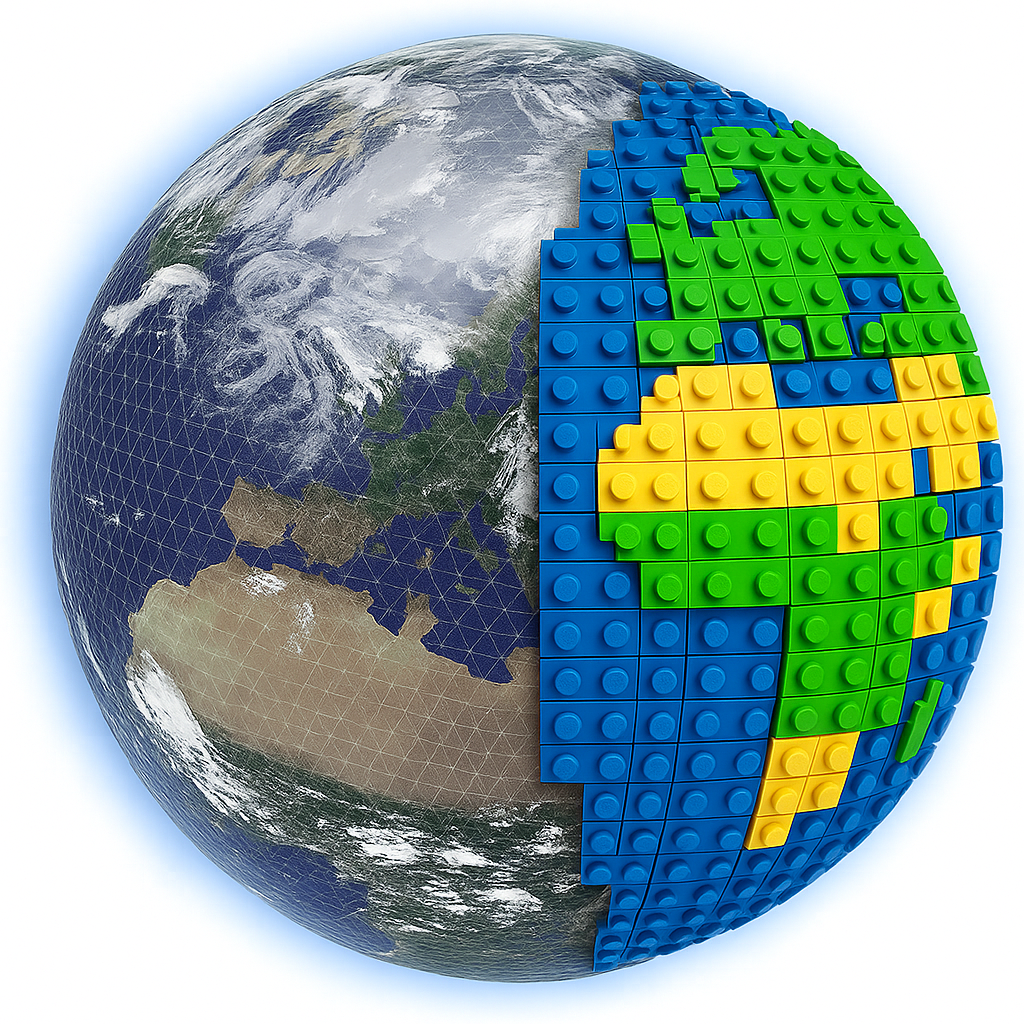
\includegraphics[width=1.4cm]{legoesm_logo.png}};

% differentiability arrow (right side, spanning the stack)
\draw[-{Latex[length=3mm]},legoSlate,line width=1.4pt]
   ($(core.south east)+(0.55,0.1)$) -- ($(ml.north east)+(0.55,-0.1)$)
   node[midway,rotate=90,above=2pt,font=\footnotesize\bfseries,text=legoSlate]{end-to-end \jaxgrad};

% composability axes (left side caption box)
\node[draw=legoSlate,rounded corners,line width=0.6pt,align=left,font=\scriptsize,
      anchor=north west,text width=4.6cm] at ($(core.south west)+(0,-0.35)$)
   {\textbf{Four composability axes}\\
    \textbullet\ \emph{grid}: cube · lat--lon · spectral · MPAS · tripole\\
    \textbullet\ \emph{complexity}: SW$\to$hydro$\to$NH; fixed-SST$\to$slab$\to$3D ocean\\
    \textbullet\ \emph{physics}: any subset of schemes, summed\\
    \textbullet\ \emph{fidelity}: idealized $\to$ AMIP/OMIP/CMIP};
\node[align=left,font=\scriptsize,anchor=north west,text width=9.7cm]
      at ($(core.south west)+(4.9,-0.35)$)
   {\textbf{One-way dependency DAG} (enforced in CI by import contracts):
    \ \texttt{core} $\prec$ \{\texttt{atmosphere}, \texttt{ocean}, \texttt{land}, \texttt{ice}\}
    $\prec$ \{\texttt{coupler}, \texttt{ml}, \texttt{tools}\}.
    Mass conserved by construction; energy/momentum tracked with explicit budget closure.
    Pure-pytree design $\Rightarrow$ \texttt{jit}/\texttt{grad}/\texttt{vmap}/\texttt{scan} through the coupled model.};
\end{tikzpicture}
\caption{\textbf{legoESM is assembled from interchangeable ``bricks''.}
The \texttt{legoesm-core} substrate (bottom) provides grids, operators, thermodynamics, time
integration, the multi-backend runtime and the differentiable parallel layer. Four
Earth-system components (atmosphere, ocean, land, ice) snap onto the core and depend only on it;
a tile-based coupler and drivers orchestrate them; the \texttt{ml} and \texttt{tools} packages
add neural operators, learned physics, differentiable training/4D-Var, forcing and diagnostics.
Because the entire stack is a pure JAX pytree, exact gradients flow end-to-end
(right). Four axes (grid, complexity, physics and fidelity) vary independently, so the same
code base runs from an LES column to a CMIP-class coupled spin-up.}
\label{fig:arch}
\end{figure*}

% =====================================================================
\section*{Many grids, one set of equations}
% =====================================================================
A central design goal is that the governing equations be solvable on whichever grid best suits
the problem. legoESM implements shallow-water, hydrostatic primitive-equation and
nonhydrostatic compressible-Euler dynamics across cubed-sphere (FV3-faithful C-D grid with
PPM transport and a duo-grid treatment of panel edges\cite{Lin2004,PutmanLin2007,Mouallem2023}),
lat--lon (C-grid finite volume\cite{Sadourny1972}), Gaussian/spectral (semi-implicit
spherical-harmonic transforms\cite{Bourke1972,HoskinsSimmons1975}) and Voronoi/MPAS
(mimetic TRiSK operators\cite{Thuburn2009,Ringler2010,Skamarock2012}) families.
Figure~\ref{fig:grids} shows the same shallow-water test (Williamson case 2, a steady
geostrophically balanced zonal jet\cite{Williamson1992}) solved on the cubed-sphere, lat--lon and
icosahedral grids: each maintains the analytic balanced flow with no spurious grid imprint over
the test period, and the cubed-sphere C-D core reproduces the Jablonowski--Williamson baroclinic
wave\cite{JablonowskiWilliamson2006} (Fig.~\ref{fig:grids}d). Removing the residual edge imprint
at cube-panel boundaries, visible only on the meridional wind and not in error norms, was one
of the problems for which the agentic ``Ralph'' loop was essential; the duo-grid sub-grid
metrics\cite{Mouallem2023} eliminate it. A complete cross-grid verification suite (cosine-bell
advection, Williamson 5 and 6, convergence rates) is given in Supplementary
Information~\S2.

\begin{figure*}[!htbp]
\centering
\begin{subfigure}{0.99\textwidth}
  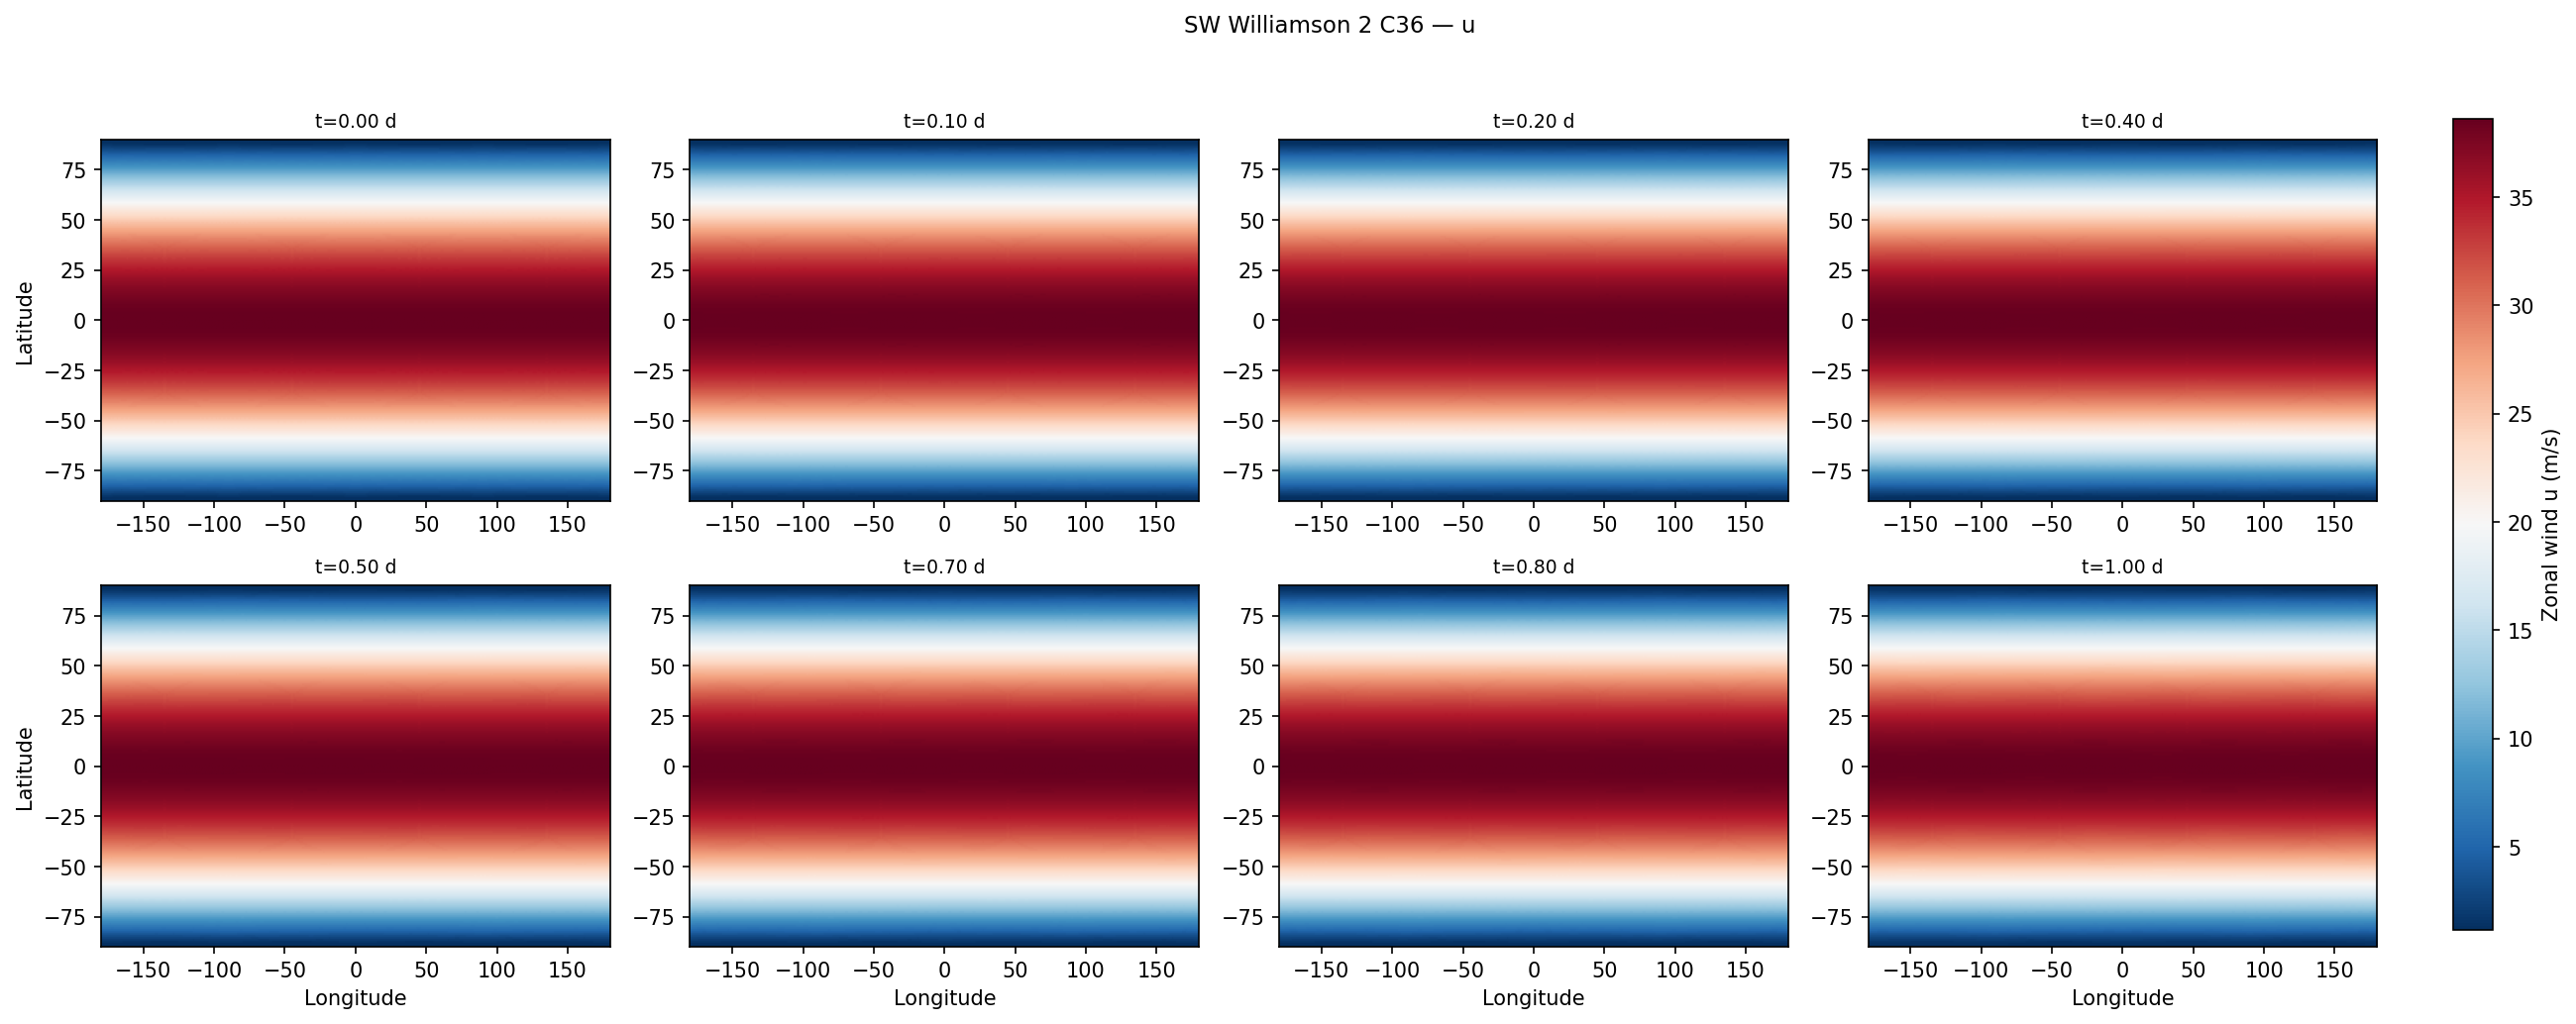
\includegraphics[width=\textwidth]{f2_sw_w2_cube.png}
  \caption{Cubed-sphere (C36)}
\end{subfigure}\\[2pt]
\begin{subfigure}{0.495\textwidth}
  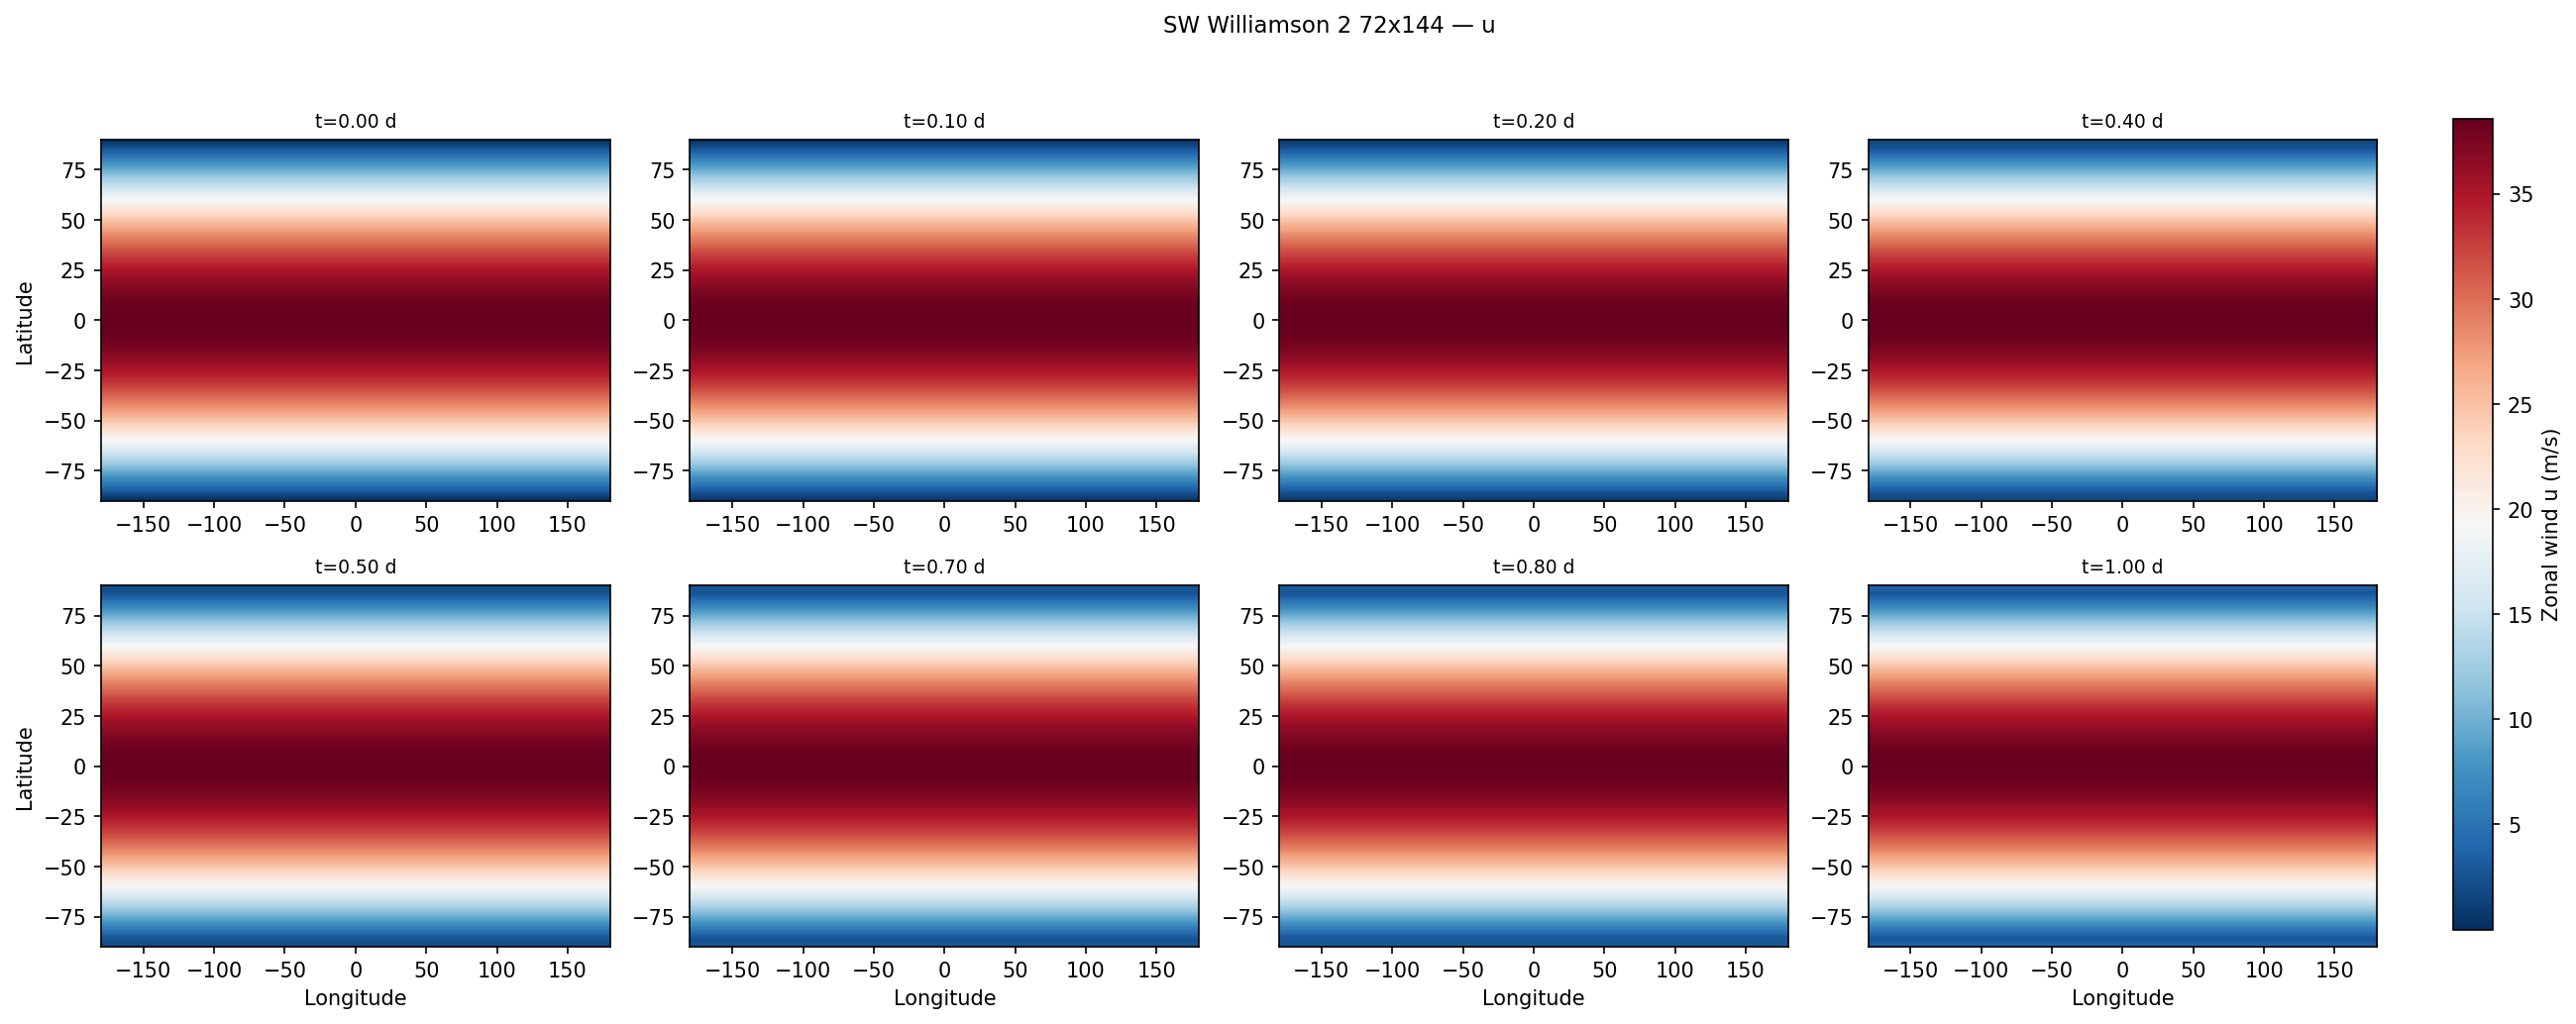
\includegraphics[width=\textwidth]{f2_sw_w2_latlon.png}
  \caption{Lat--lon (72$\times$144)}
\end{subfigure}\hfill
\begin{subfigure}{0.495\textwidth}
  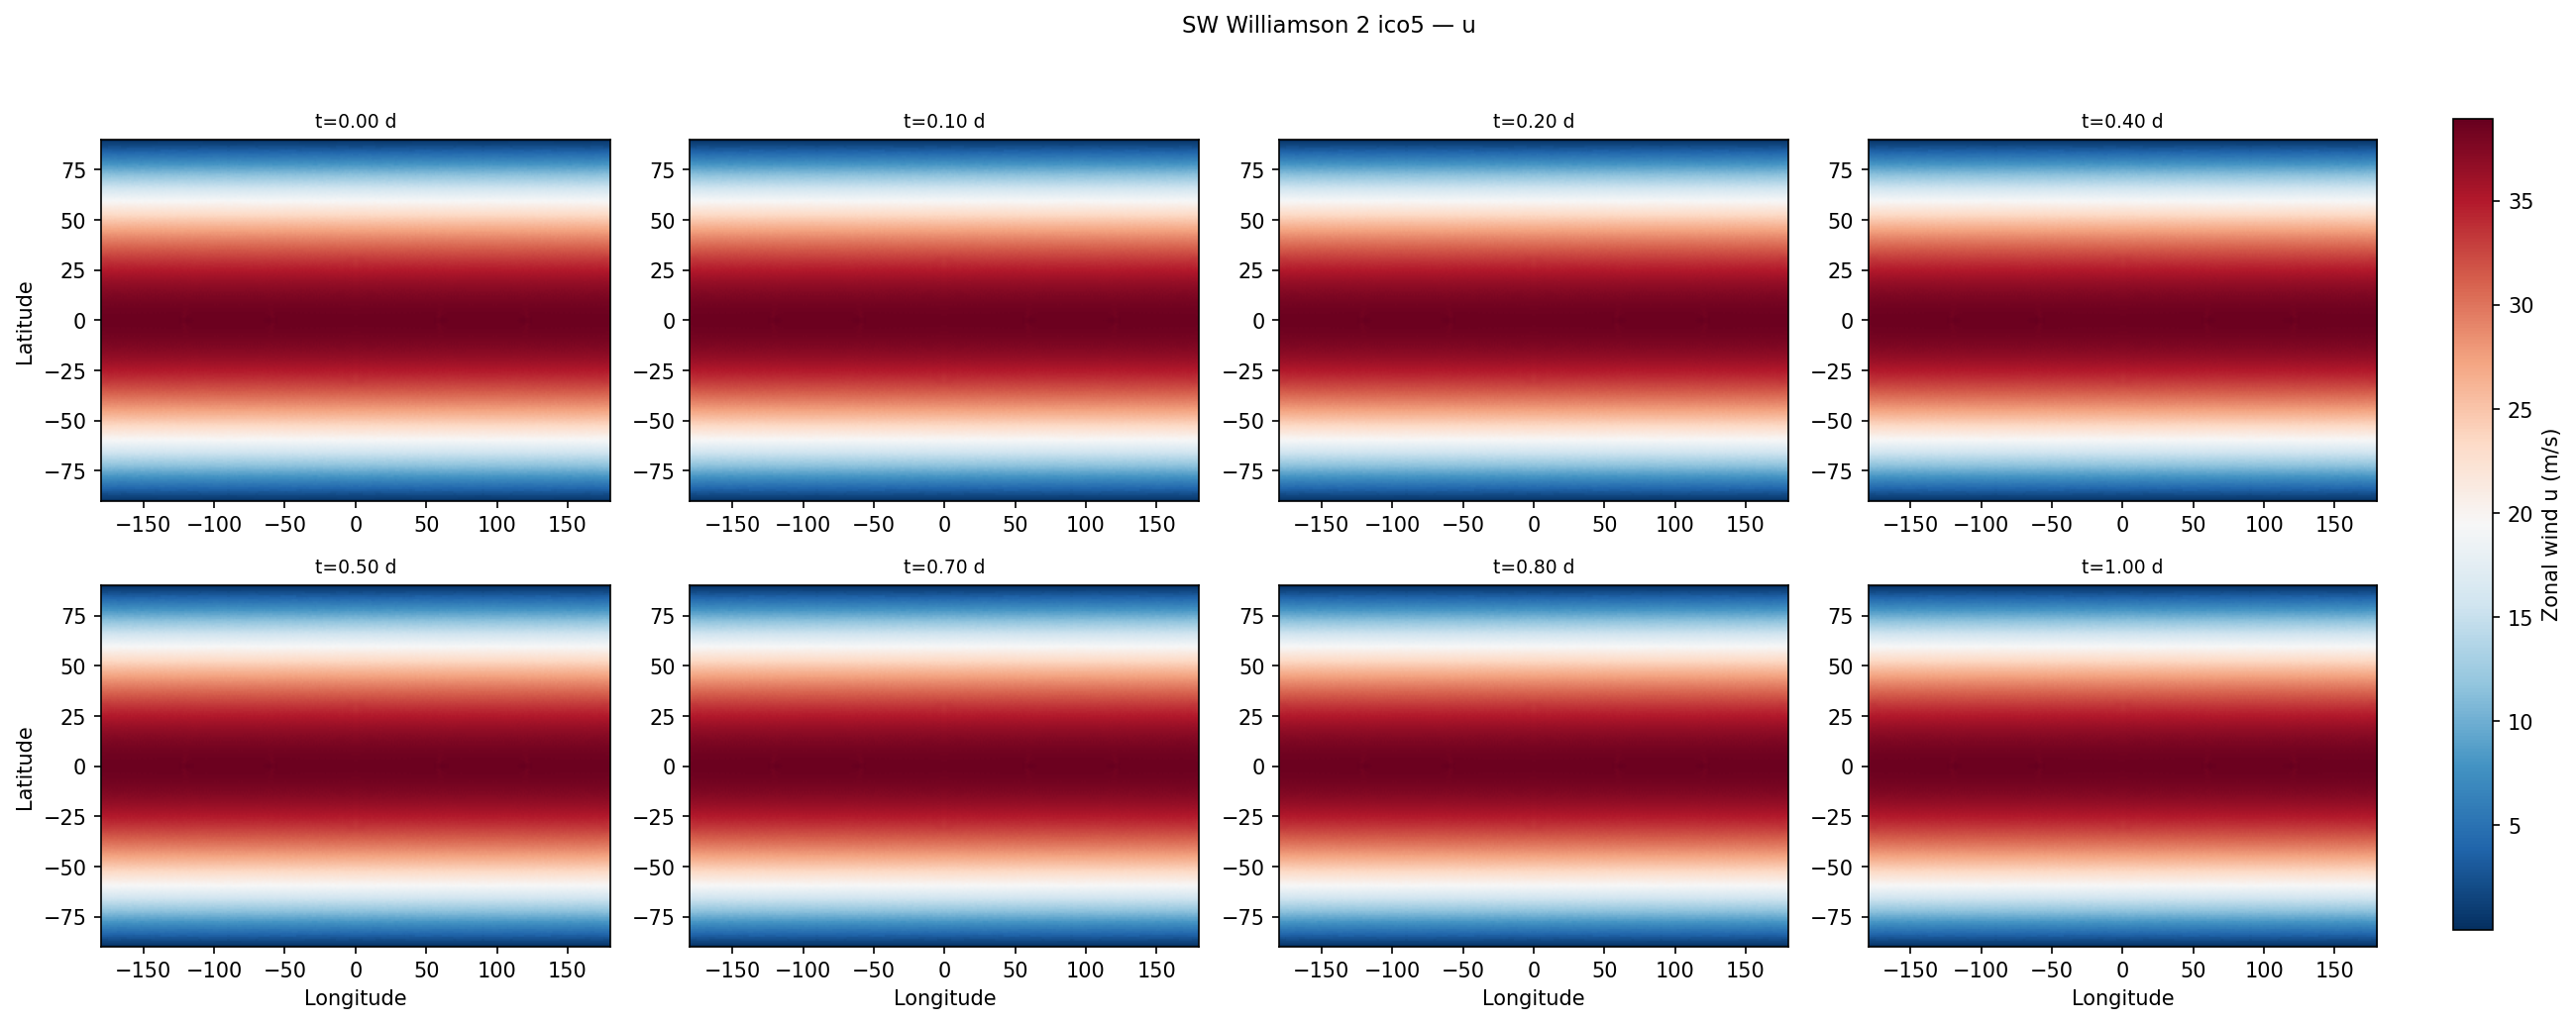
\includegraphics[width=\textwidth]{f2_sw_w2_ico.png}
  \caption{Icosahedral (ico5)}
\end{subfigure}\\[3pt]
\begin{subfigure}{0.99\textwidth}
  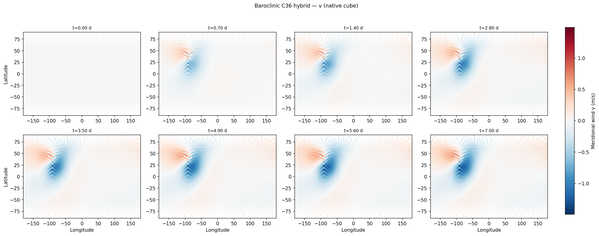
\includegraphics[width=\textwidth]{f2_baroclinic_v_cube.jpg}
  \caption{Jablonowski--Williamson baroclinic wave, meridional wind, cubed-sphere C36 (native panels)}
\end{subfigure}
\caption{\textbf{One equation set on many grids.}
(a--c) The Williamson-2 steady balanced zonal jet (shallow-water zonal wind $u$, m\,s$^{-1}$)
integrated on three grid families; the balanced state is maintained on each without grid-scale
noise. (d) The Jablonowski--Williamson baroclinic-instability test on the FV3-faithful
cubed-sphere C-D core, shown on the six native cube panels: the wave develops cleanly across
panel edges. The numerical method (discretization) and the physical equation set are orthogonal
choices in legoESM. See Supplementary Information~\S2 for the full cross-grid suite and
convergence rates.}
\label{fig:grids}
\end{figure*}

% =====================================================================
\section*{Composability and differentiable calibration}
% =====================================================================
Swapping one physical scheme for another to assess its effect is a routine scientific need,
yet it is difficult in conventional climate models, in which parameterizations are interwoven
with the rest of the code. In legoESM, every parameterization presents the same interface,
taking the atmospheric state and returning a tendency, so schemes can be exchanged without
modifying the rest of the model. Figure~\ref{fig:compdiff}a,b illustrates this for atmospheric
convection, the moist rising motions that produce most tropical rainfall and a long-standing
source of model error. Ten different convection schemes (Bechtold, Tiedtke,
Kain--Fritsch, Zhang--McFarlane\cite{ZhangMcFarlane1995}, Emanuel, Kuo, a unified mass-flux
scheme, and others) are each run, unchanged, in a single atmospheric column held in
radiative--convective equilibrium (a small, well-understood testbed) and scored against the
temperature profile that theory predicts. They separate cleanly by skill
(Fig.~\ref{fig:compdiff}b), recovering the expected ordering and exposing which ones fail to
reach equilibrium: an experiment that is cumbersome in a conventional model but a one-line
change here. The same mechanism can replace an entire component: a classical physics suite, a
column neural network, or a full spherical neural operator\cite{Bonev2023} (a learned
dynamical core) can occupy the same slot, and the ocean can run as a prescribed sea surface,
a simple slab, or a full three-dimensional model, all from one driver (Supplementary
Information~\S3).

Differentiability turns calibration into gradient descent. Because gradients flow through the
coupled model via \jaxgrad{}, uncertain parameters can be optimized directly against data with
modern optimizers, rather than by derivative-free search\cite{Hourdin2017,Cleary2021}.
Figure~\ref{fig:compdiff}c demonstrates this for the land surface: tuning per-plant-functional-type
soil-water and surface parameters by gradient descent against ERA5\cite{Hersbach2020}
skin temperature, under physical-bound constraints imposed through differentiable
transforms, reduces the global annual-mean warm bias from $+3.11$ to $+1.80$\,K and the RMSE
from $4.44$ to $3.01$\,K, with the largest improvements over the previously too-warm tropical
land. The same machinery has been used to calibrate convection-scheme parameters against
cloud-resolving references, and to adjust a cloud-fraction critical-relative-humidity threshold
using gradients of the top-of-atmosphere shortwave and longwave fluxes so that the planetary
albedo falls in its observed $\sim$30\% range. The differentiable parallel layer makes this
work at scale: exact reverse-mode gradients flow through distributed halo exchange (via a custom
adjoint that swaps send/receive ranks) and through the global reductions used by the
mass-conservation fixers (Methods).

\begin{figure*}[!htbp]
\centering
\begin{subfigure}{0.62\textwidth}
  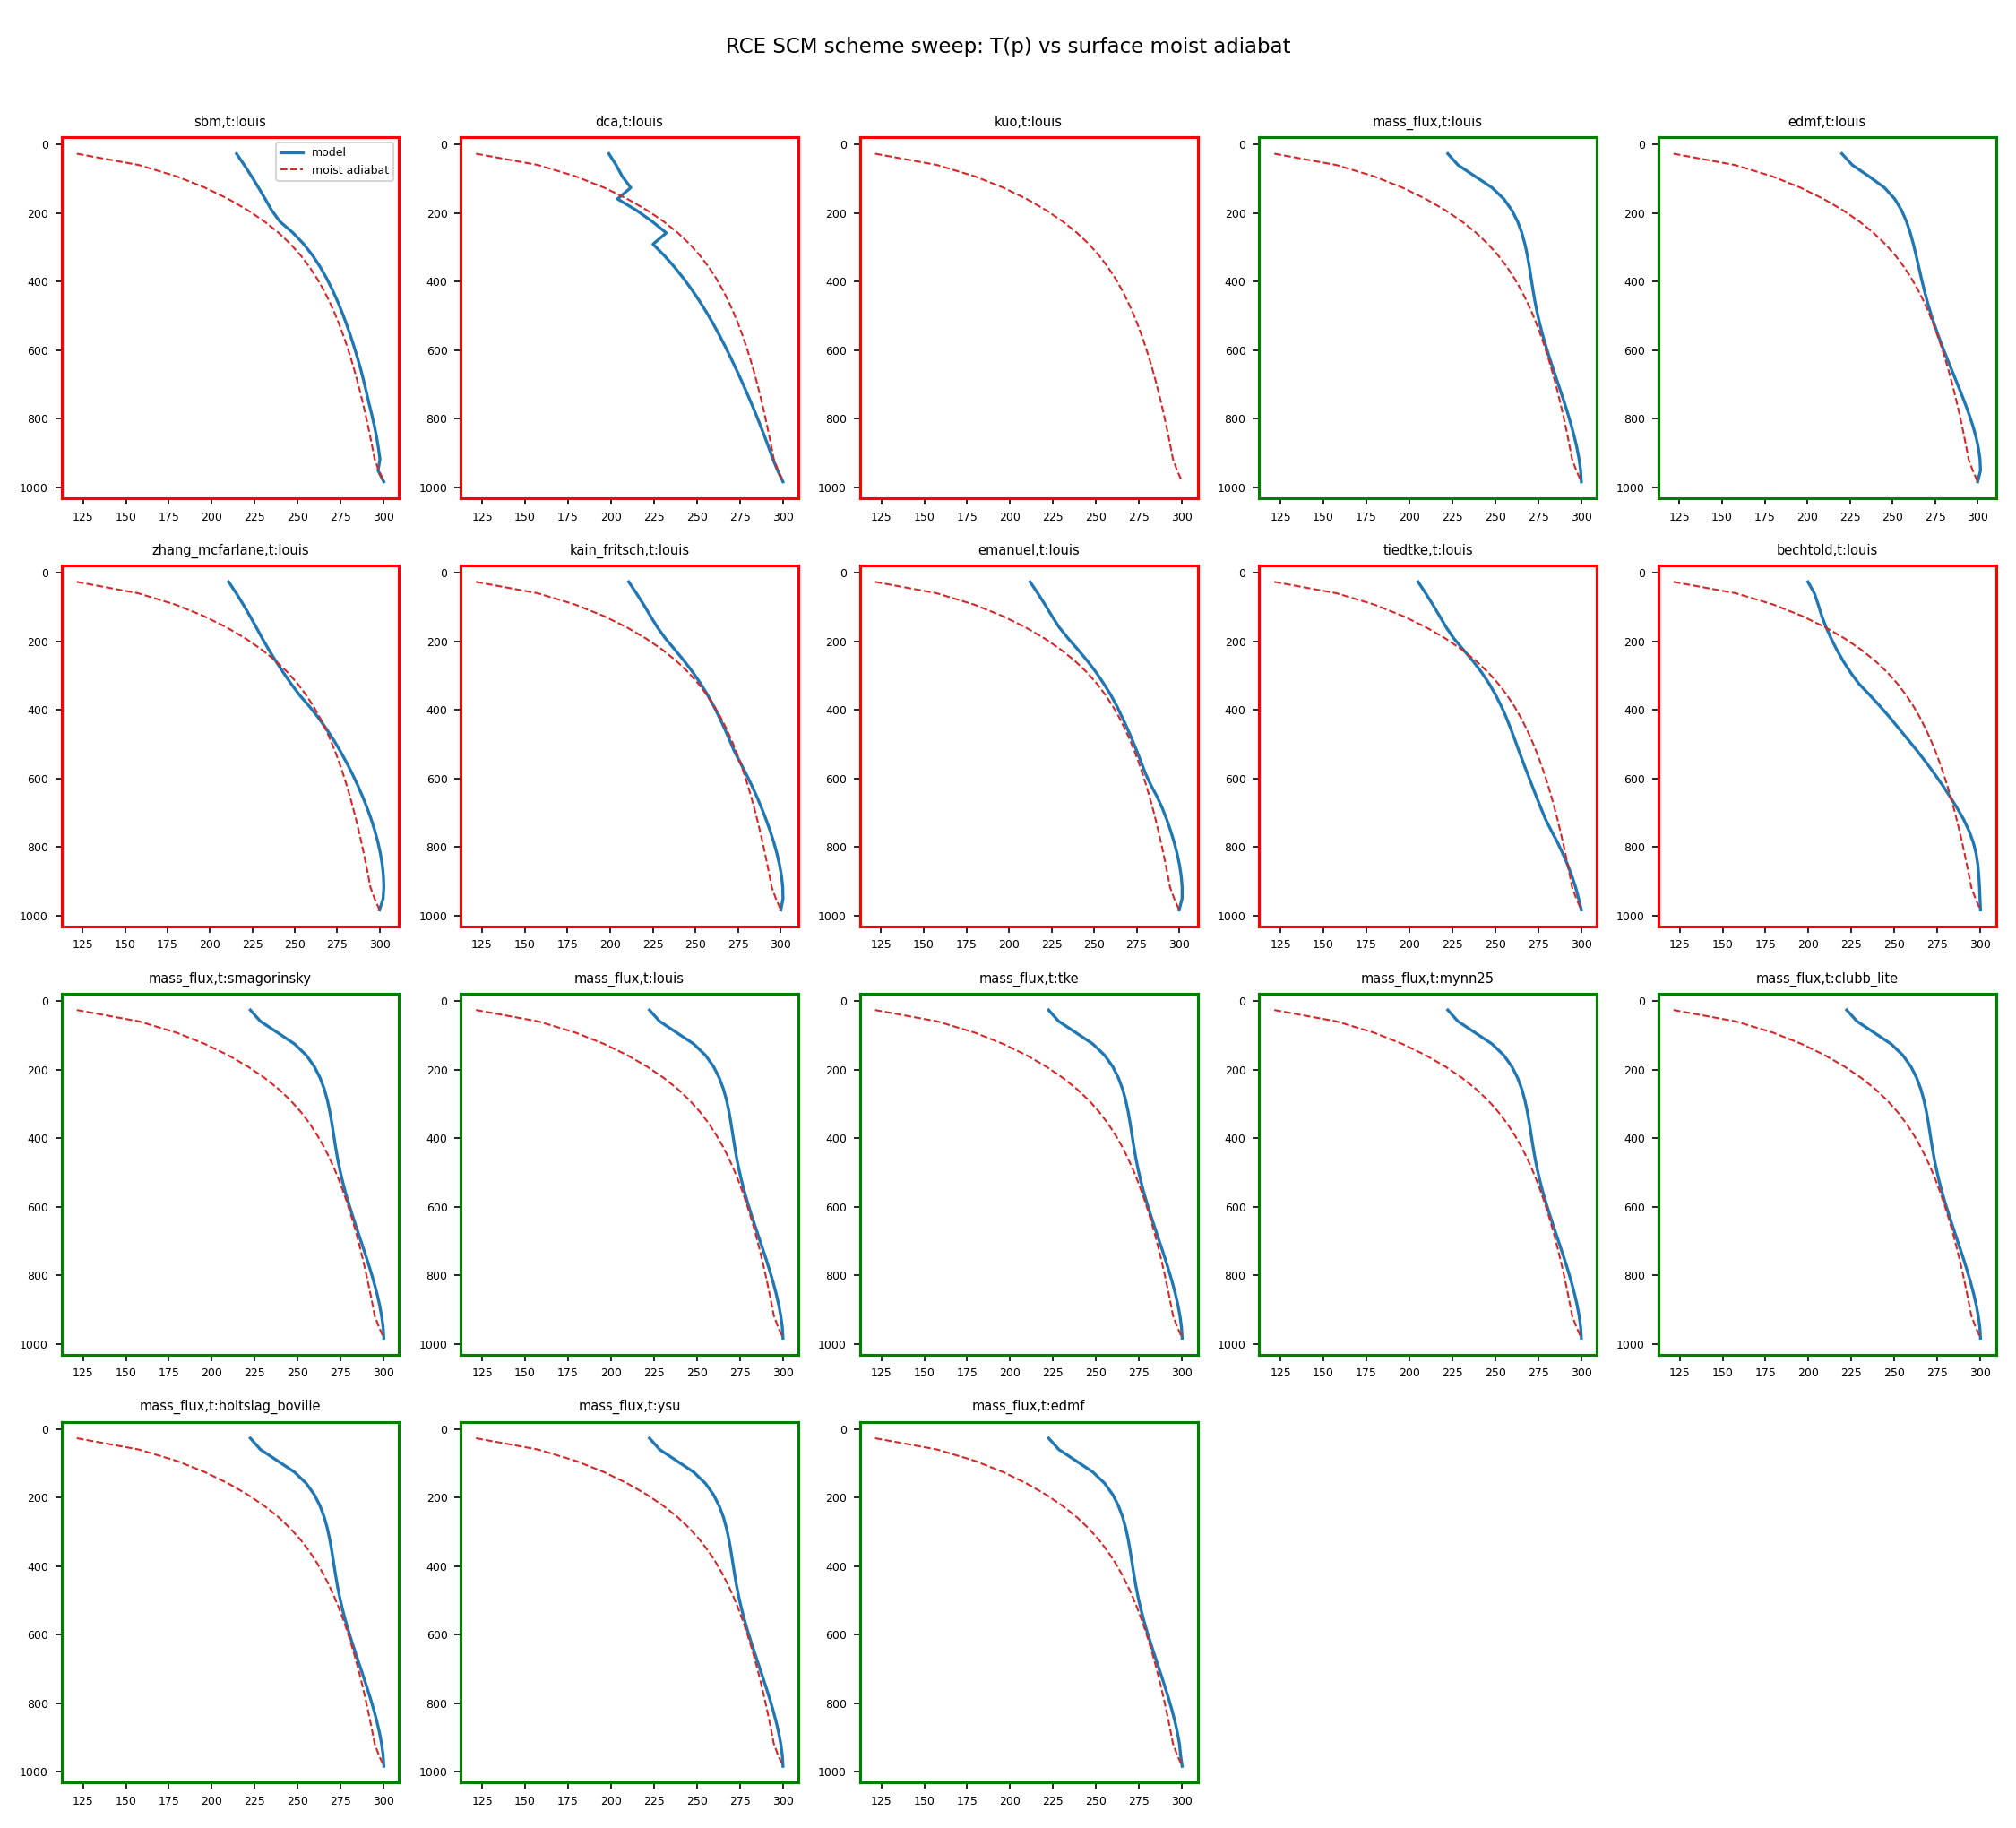
\includegraphics[width=\textwidth]{f3_conv_sweep.png}
  \caption{Convection schemes in RCE vs.\ moist-adiabat oracle}
\end{subfigure}\hfill
\begin{subfigure}{0.36\textwidth}
  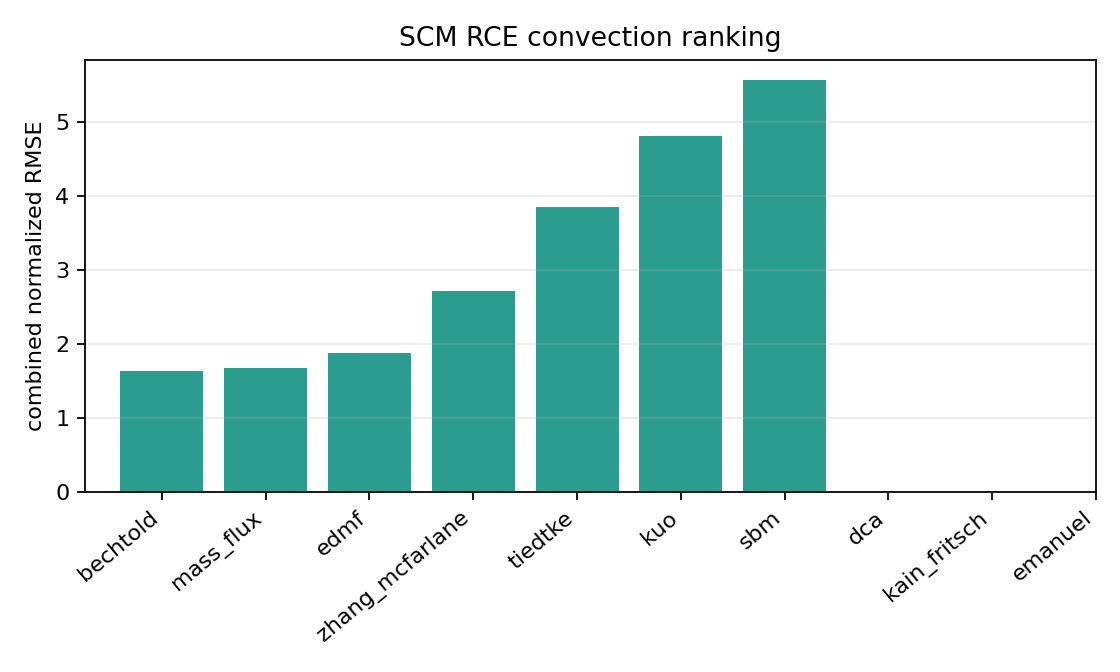
\includegraphics[width=\textwidth]{f3_conv_ranking.png}
  \caption{Skill ranking}
\end{subfigure}\\[4pt]
\begin{subfigure}{0.99\textwidth}
  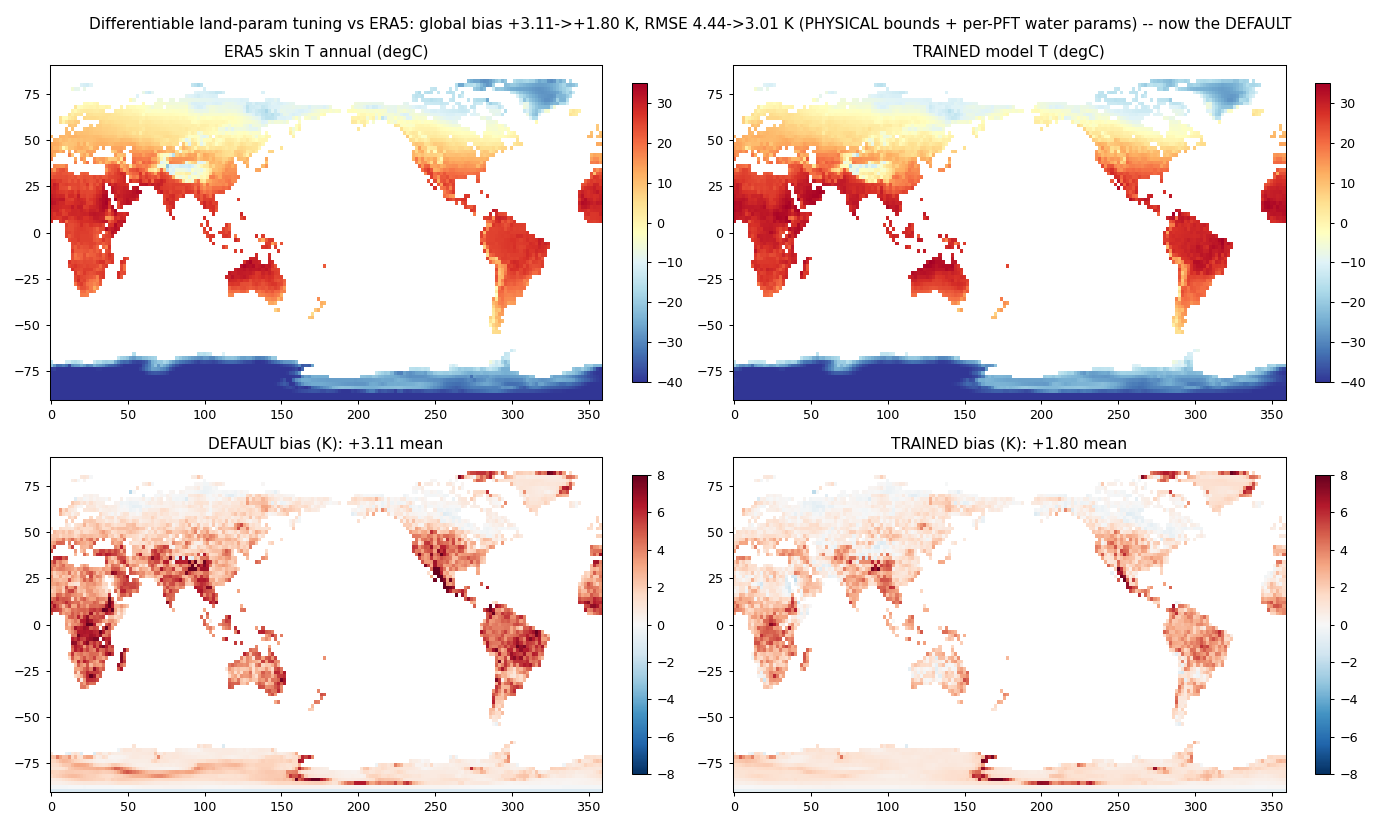
\includegraphics[width=\textwidth]{f3_land_tuning.png}
  \caption{Differentiable land-parameter calibration against ERA5 skin temperature}
\end{subfigure}
\caption{\textbf{Composability and differentiable calibration.}
(a) Ten convection parameterizations, each swapped unchanged into a single-column RCE setup,
compared against the surface moist adiabat (temperature profiles; green/red frames mark
pass/fail of the equilibrium realism gate). (b) Combined normalized RMSE ranks the schemes by
skill. (c) Gradient-descent calibration of per-plant-functional-type land parameters against
ERA5 skin temperature reduces the global-mean bias from $+3.11$ to $+1.80$\,K and the RMSE from
$4.44$ to $3.01$\,K (left: ERA5 and trained model; right: bias maps before and after). Gradients
are obtained by differentiating the coupled model end-to-end.}
\label{fig:compdiff}
\end{figure*}

% =====================================================================
\section*{Bridging scales, from turbulence to the globe}
% =====================================================================
Climate processes span an enormous range of scales, from turbulent eddies metres across to
circulations spanning the planet, and traditionally each scale is treated with a separate
model. legoESM covers this range within a single framework. On a small
doubly periodic domain, its nonhydrostatic core with a turbulence closure\cite{Smagorinsky1963}
performs large-eddy simulation, resolving the largest turbulent motions directly: the canonical
GABLS1 stable boundary layer\cite{Beare2006} (Fig.~\ref{fig:multiscale}a), the Ekman layer, the
Wangara diurnal cycle, and the DYCOMS-II\cite{Stevens2005} and RICO\cite{vanZanten2011}
cloud-topped layers all reproduce the expected mean profiles and turbulence structure
(Supplementary Information~\S4). Enlarging the domain and adding moist physics turns the same
core into a cloud-resolving model: in radiative--convective equilibrium\cite{Wing2018} it
spontaneously organizes convection into clusters (``self-aggregation'',
Fig.~\ref{fig:multiscale}b), and its warm-rain microphysics matches a benchmark
particle-based reference\cite{Shima2009,Bartman2022} (Supplementary Information~\S4). At the
global scale, the cubed-sphere atmosphere runs prescribed-ocean (AMIP-style) simulations and
the three-dimensional ocean runs forced (OMIP-style) integrations (next section). Spanning a
metre-scale eddy to a global simulation within one differentiable code base is, to our
knowledge, unique, and it is precisely what hybrid physics--AI modelling needs, since the
high-resolution end can generate training data and the global end can host the learned scheme.

\begin{figure*}[!htbp]
\centering
\begin{subfigure}{0.46\textwidth}
  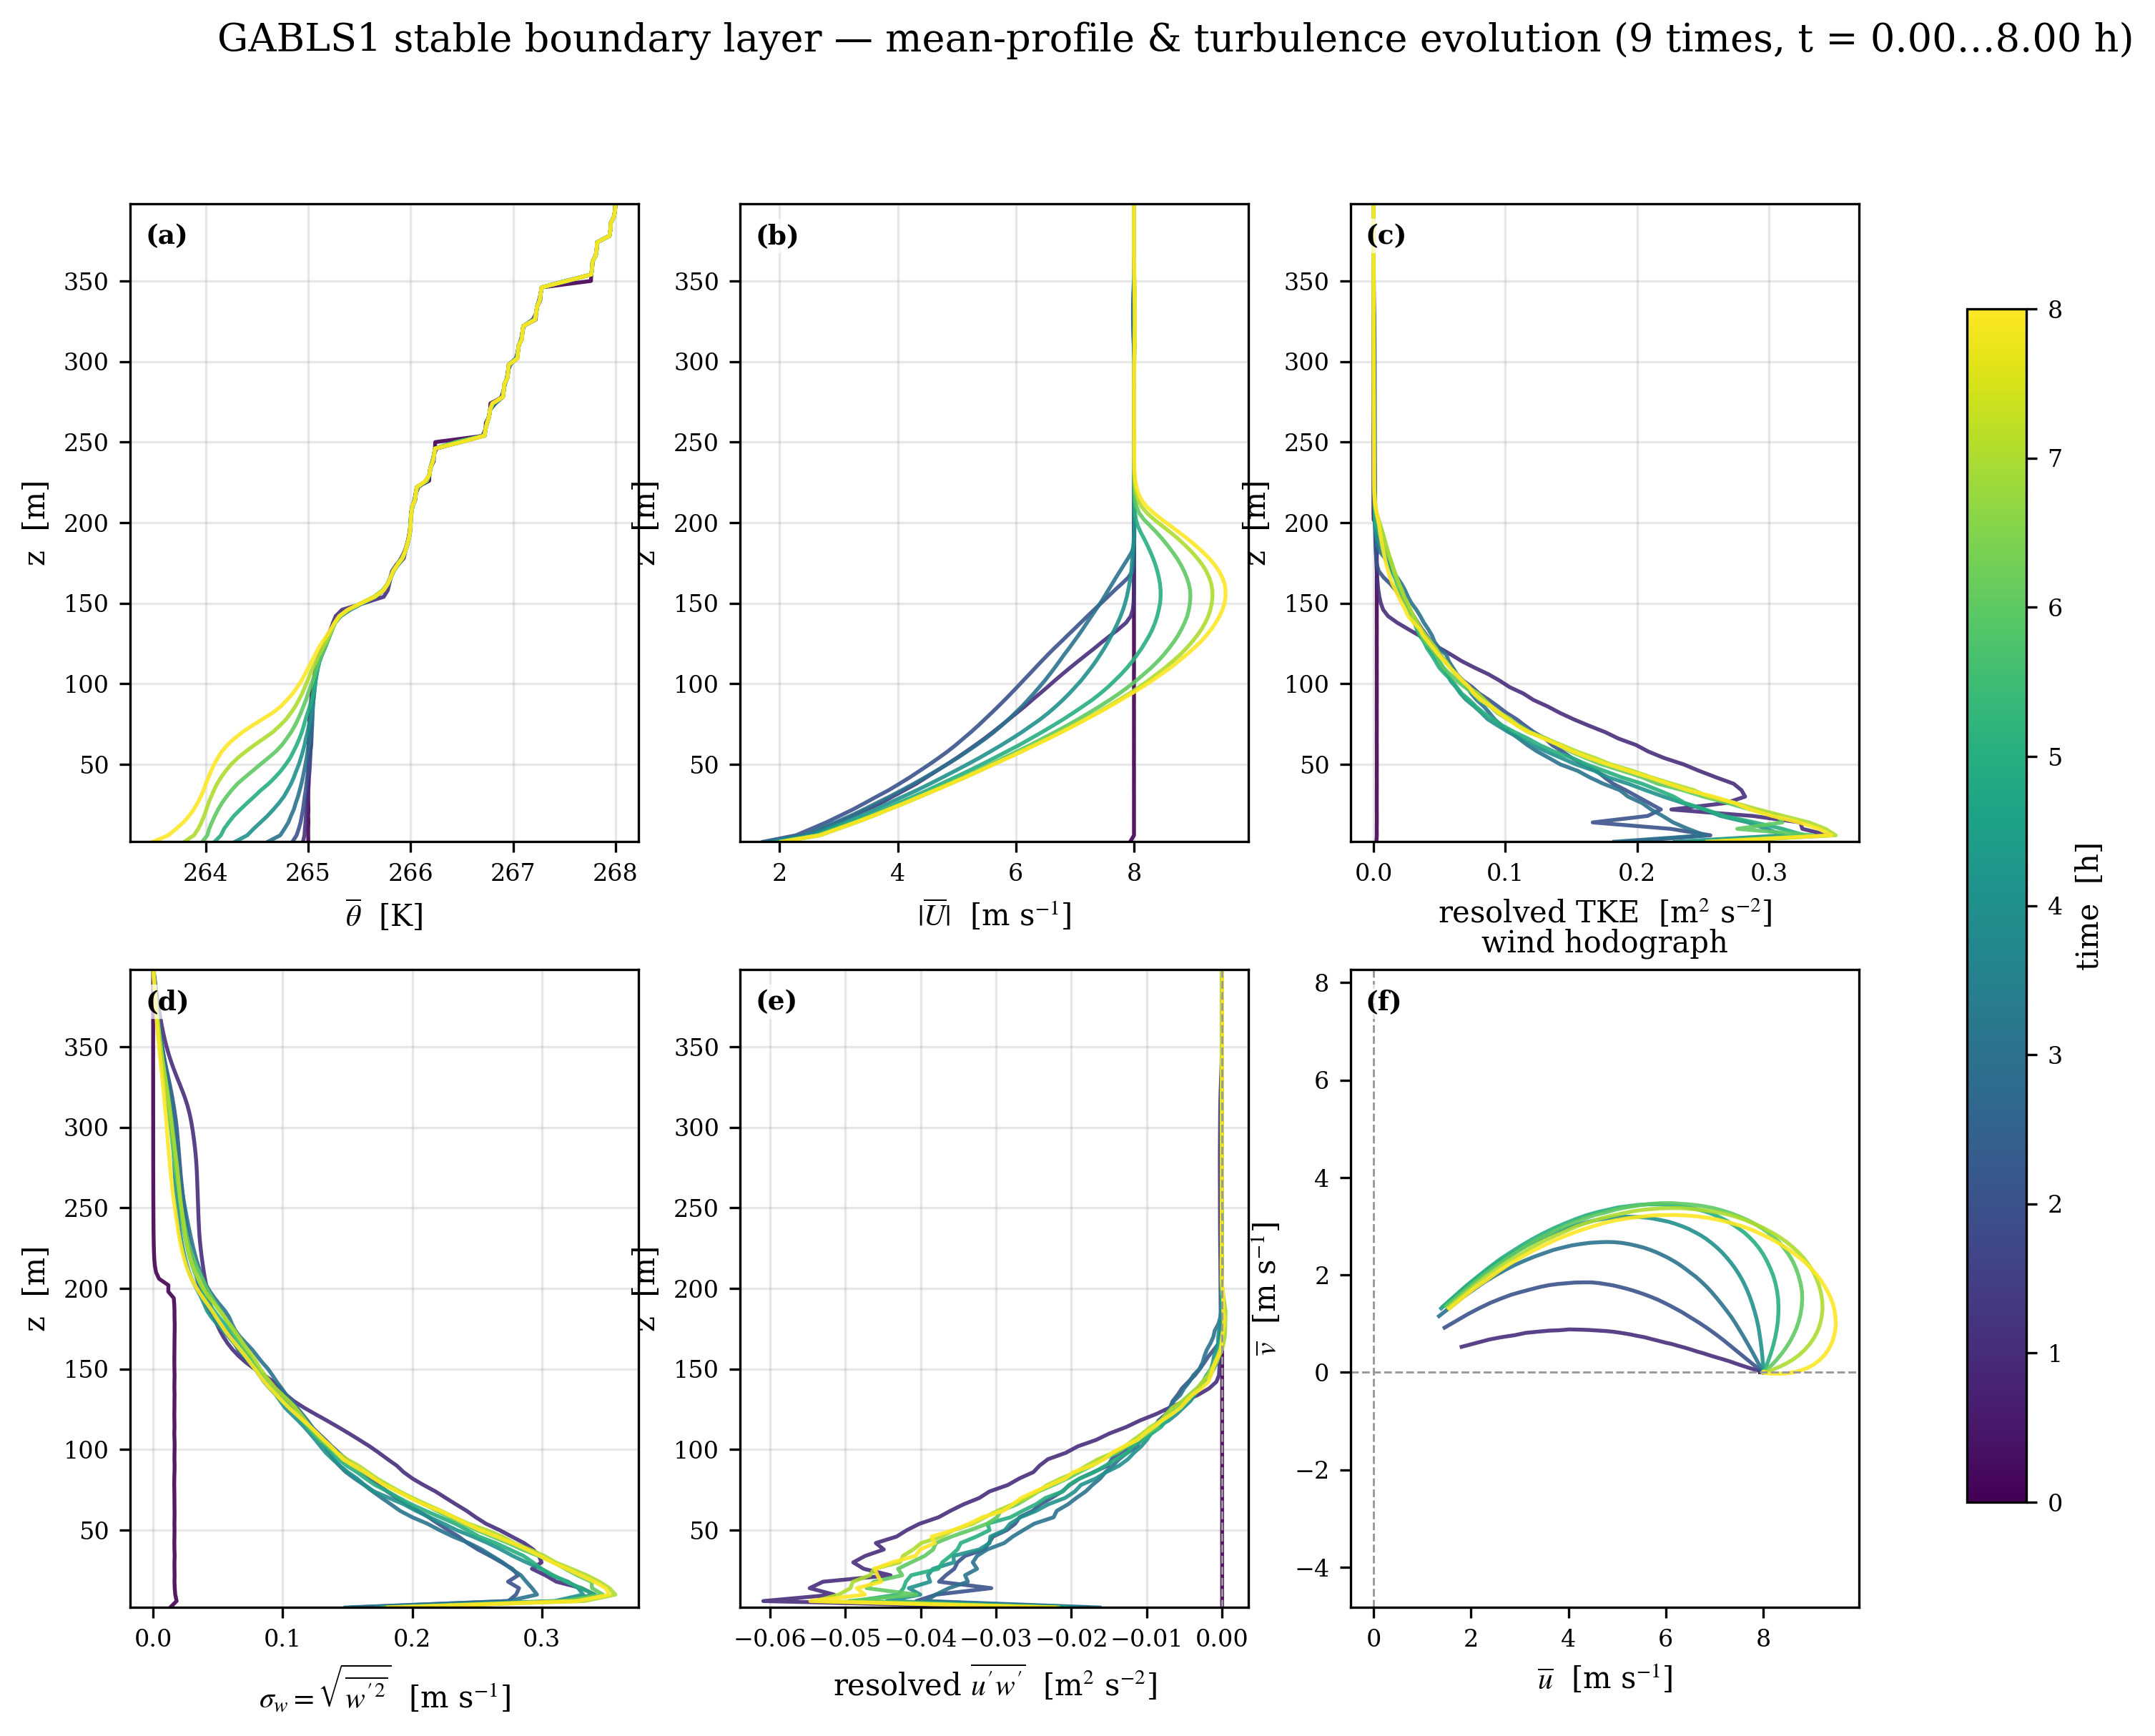
\includegraphics[width=\textwidth]{f4_les_gabls1.png}
  \caption{LES: GABLS1 stable boundary layer}
\end{subfigure}\hfill
\begin{subfigure}{0.52\textwidth}
  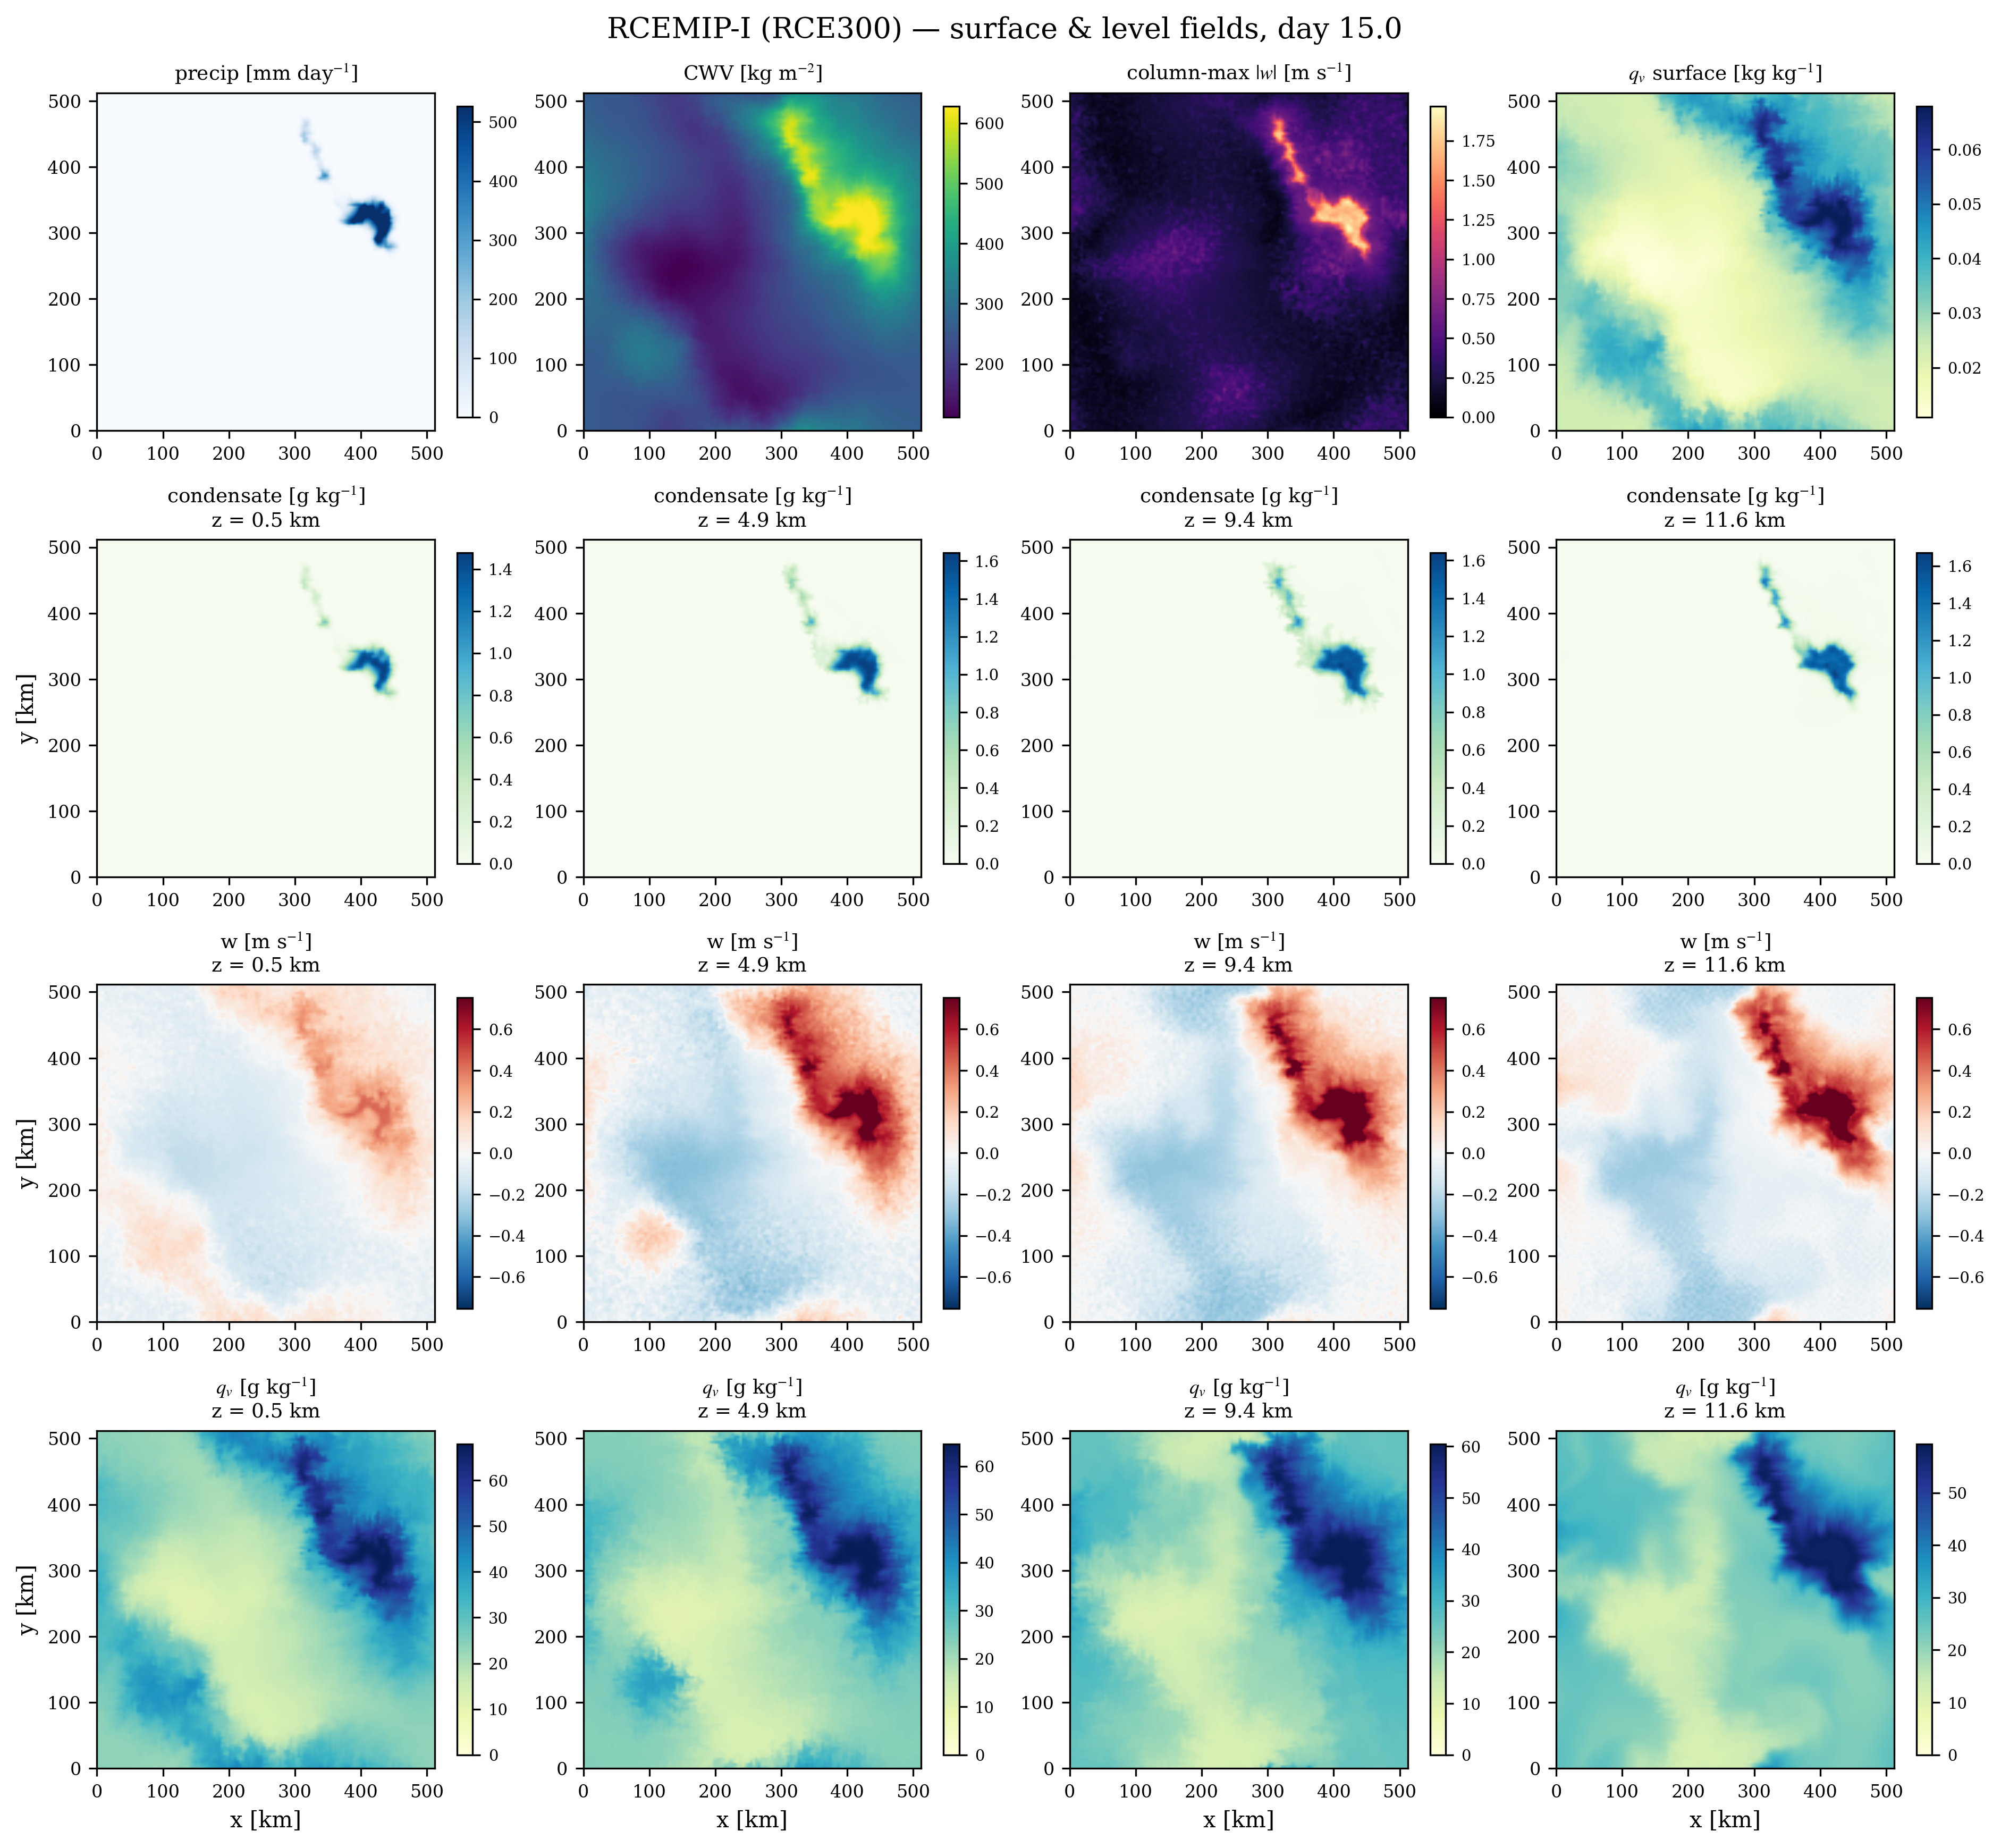
\includegraphics[width=\textwidth]{f4_crm_rcemip.png}
  \caption{CRM: RCEMIP self-aggregation (day 15)}
\end{subfigure}
\caption{\textbf{Bridging scales within one code base.}
(a) Large-eddy simulation of the GABLS1 stable boundary layer (time evolution of mean wind,
potential temperature and turbulence), using the nonhydrostatic plane core with a dynamic
Smagorinsky closure. (b) Cloud-resolving radiative--convective equilibrium (RCEMIP RCE300):
surface and level fields after 15 days show spontaneous convective self-aggregation.
The same parameterization interfaces and dynamical cores are used from LES through CRM to global
configurations; see Supplementary Information~\S4 for the full LES/CRM suites.}
\label{fig:multiscale}
\end{figure*}

% =====================================================================
\section*{A global ocean across complex grids}
% =====================================================================
A stringent test of the framework is whether its ocean component, built from the same
composable elements, can reproduce a mature community model on the complex grids used in
operational ocean modelling. The three-dimensional ocean solves the same primitive equations as established
models, with a split-explicit free-surface solver\cite{ShchepetkinMcWilliams2005}, KPP vertical
mixing\cite{LMD1994} and Gent--McWilliams eddy transport\cite{GM1990}, and runs on
latitude--longitude, cubed-sphere, unstructured (MPAS/Voronoi) and NEMO-style tripolar grids.
Figure~\ref{fig:ocean} compares legoESM ocean integrations against
NEMO\cite{Madec2017} on two of the most demanding meshes. On the unstructured MPAS/Voronoi
icosahedral grid, the simulated sea-surface temperature and the zonal-mean temperature section
closely track NEMO across the global domain and the full water column
(Fig.~\ref{fig:ocean}a,b). On the tripolar grid, whose folded northern boundary is a classic
source of numerical artifacts, the modelled sea-surface height matches the NEMO field with a
spatial correlation of 0.95 and near-zero bias (Fig.~\ref{fig:ocean}c). A centennial spin-up
library, an AMOC tracker, conservation diagnostics, and a peer-comparison fidelity harness
support quantitative model intercomparison (Supplementary Information~\S5). That an
agent-built ocean reproduces a mature community model on its own native, geometrically awkward
grids is a strong test of the framework.

\begin{figure*}[!htbp]
\centering
\begin{subfigure}{0.99\textwidth}
  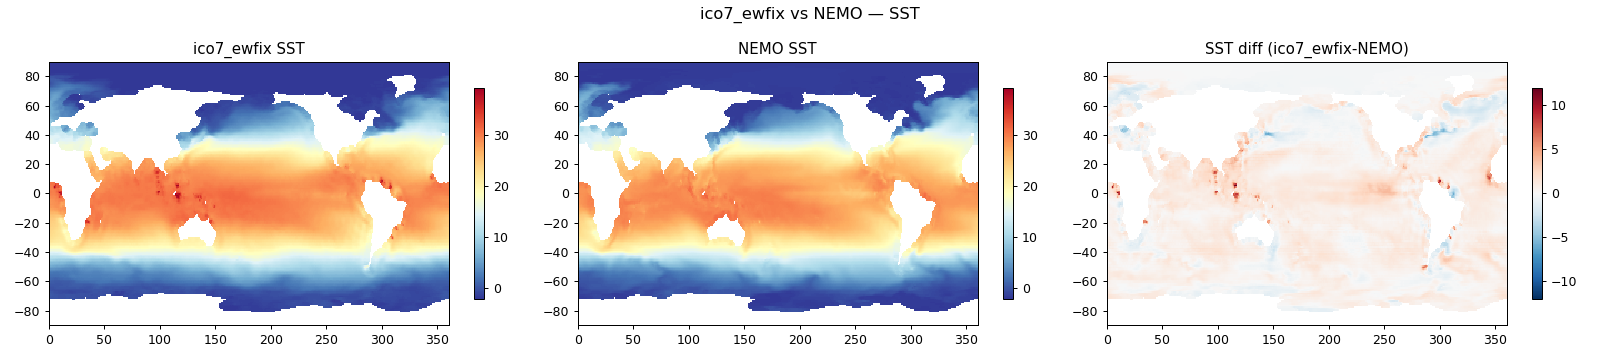
\includegraphics[width=\textwidth]{f5_ocean_mpas_sst.png}
  \caption{MPAS/Voronoi (icosahedral) sea-surface temperature vs.\ NEMO}
\end{subfigure}\\[3pt]
\begin{subfigure}{0.62\textwidth}
  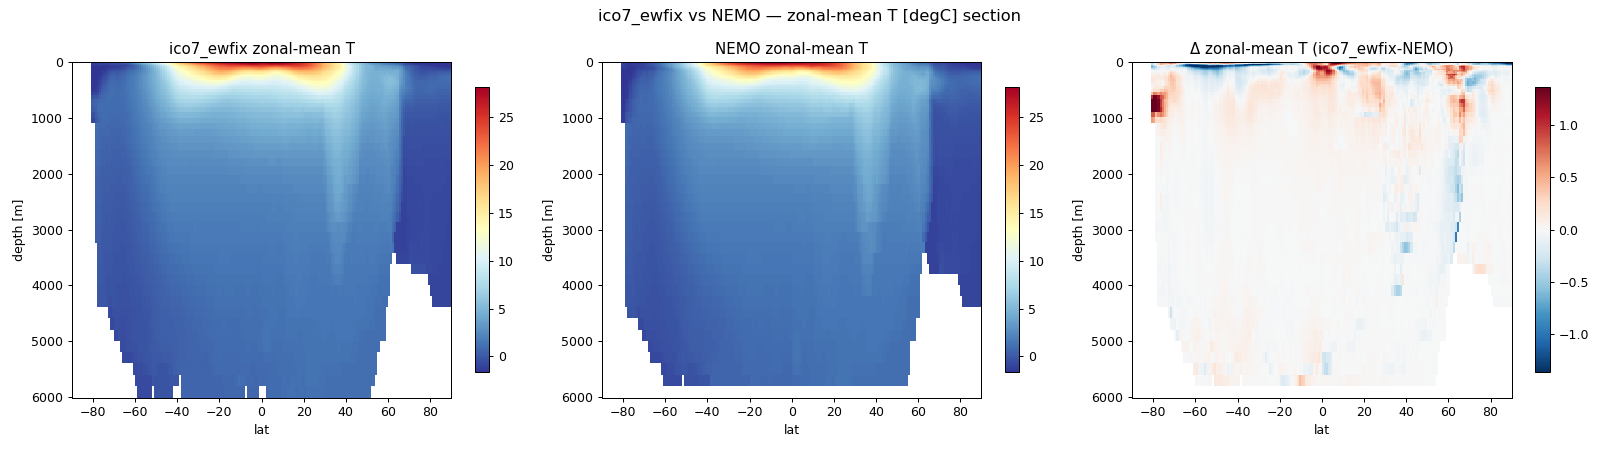
\includegraphics[width=\textwidth]{f5_ocean_mpas_tsection.png}
  \caption{Zonal-mean temperature section vs.\ NEMO}
\end{subfigure}\hfill
\begin{subfigure}{0.36\textwidth}
  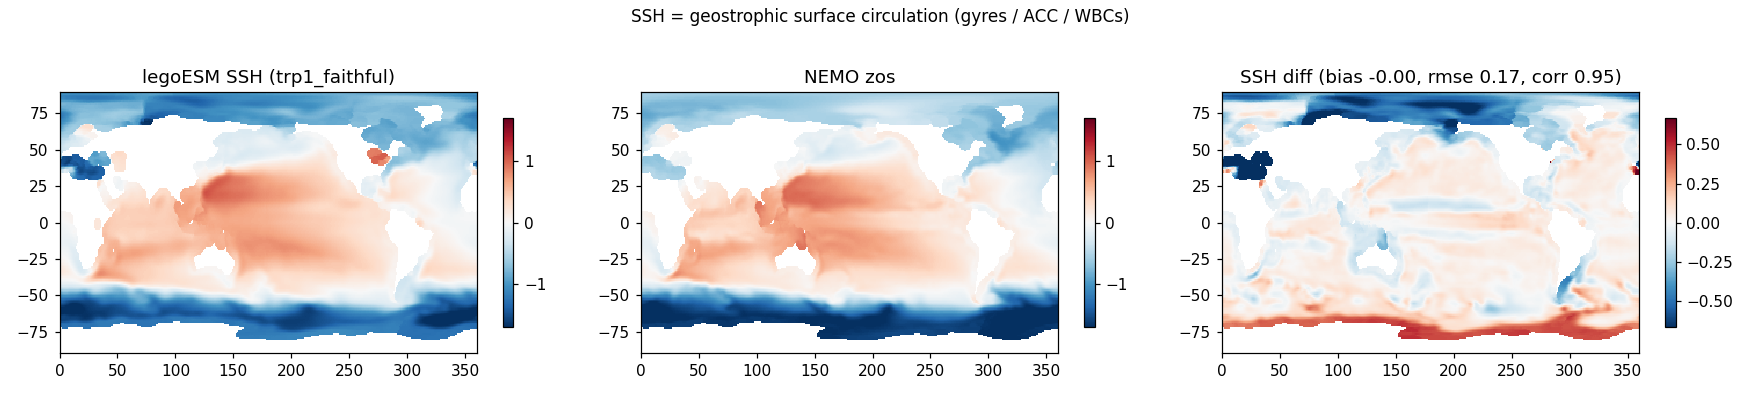
\includegraphics[width=\textwidth]{f5_ocean_tripole_ssh.png}
  \caption{Tripolar SSH vs.\ NEMO ($r=0.95$)}
\end{subfigure}
\caption{\textbf{A global ocean validated against NEMO on complex grids.}
(a) Sea-surface temperature and (b) zonal-mean temperature section from the legoESM ocean on the
unstructured MPAS/Voronoi icosahedral grid, against NEMO, with difference maps. (c) Sea-surface
height on the NEMO-style tripolar (eORCA) grid reproduces the NEMO field with spatial correlation
$r=0.95$ and bias $\approx 0$, despite the folded northern boundary. Full ocean diagnostics,
additional grids and the fidelity harness are in Supplementary Information~\S5.}
\label{fig:ocean}
\end{figure*}

% =====================================================================
\section*{Performance and scalability}
% =====================================================================
Practical use requires that the model run efficiently for the long integrations and large
ensembles needed to characterize variability and extremes, and on whatever hardware is
available. Writing legoESM in JAX makes it portable and fast without hand-written accelerator code.
A single consumer GPU accelerates the atmosphere by $16$--$21\times$ and the ocean by
$33$--$99\times$
over a 24-core CPU at single precision (Fig.~\ref{fig:scaling}a,b), with structured grids
(lat--lon, cubed-sphere) outperforming unstructured (MPAS) and spectral cores, as expected from
memory-access patterns. Two algorithmic changes found during agentic optimization dominate the
gains: parallelizing the correlated-$k$ radiation over its $g$-points ($\sim$6$\times$ on the
radiation kernel) and a split-explicit barotropic ocean solver that escapes the global-reduction
latency wall of the implicit solver (up to $1.65\times$ faster at 64 ranks). Across MPI ranks
and nodes the model scales well where communication is amortized: the ocean reaches near-ideal
parallel efficiency at production tile sizes, and the MPAS atmosphere strong-scales to
$0.69$ efficiency at 32 ranks (Fig.~\ref{fig:scaling}c,d). Reverse-mode differentiability is
preserved across all of this: gradients flow correctly through MPI halo exchange and global
sum reductions, verified against single-rank references to machine precision (Methods). Honest
limits are documented (spectral transforms remain communication-bound, and cross-node
cube-panel exchange on a commodity TCP fabric anti-scales) and are reported in Supplementary
Information~\S6 rather than hidden.

\begin{figure*}[!htbp]
\centering
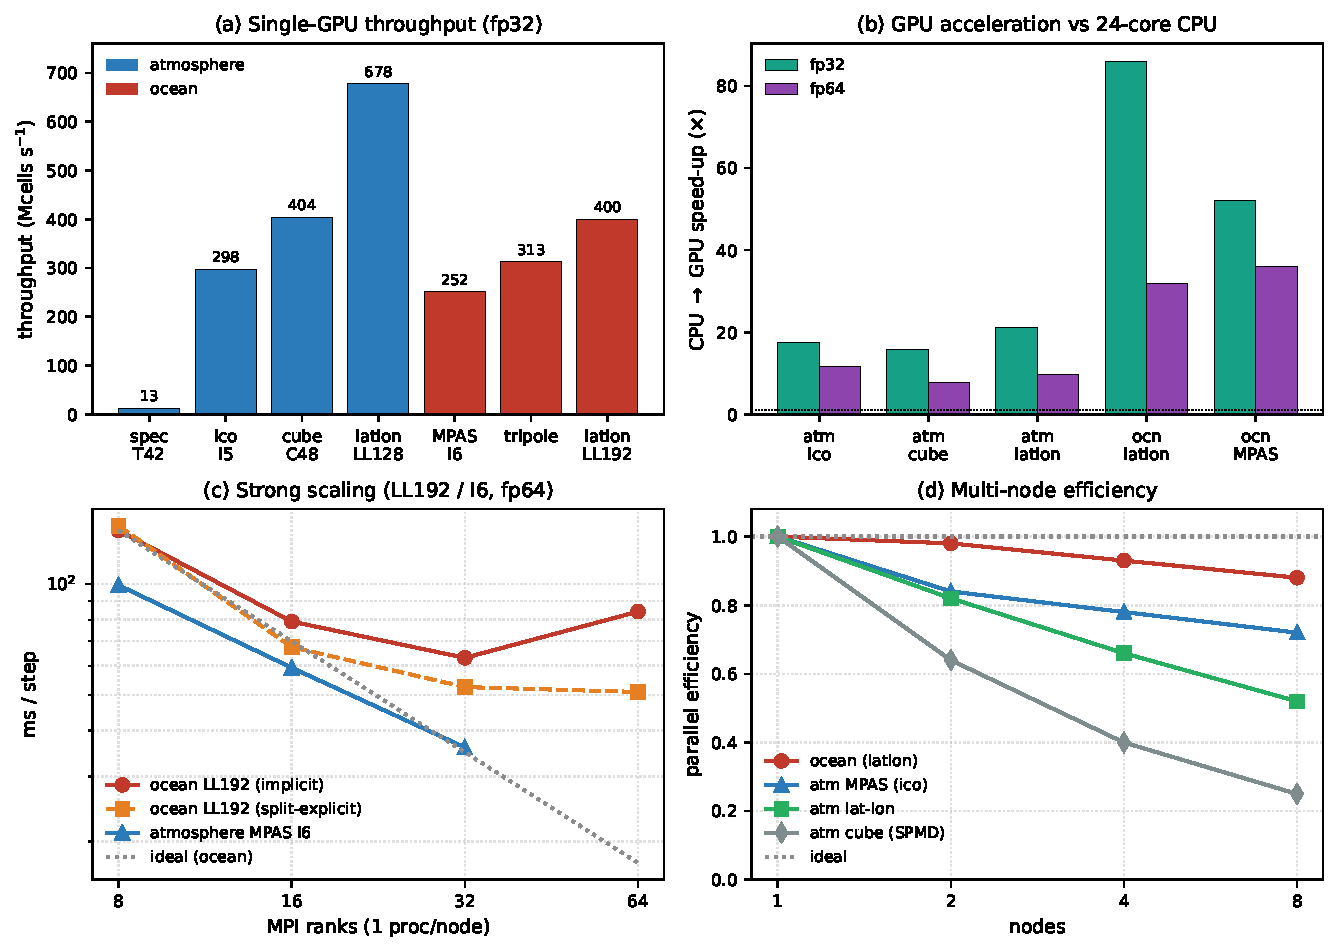
\includegraphics[width=0.96\textwidth]{f6_scaling.pdf}
\caption{\textbf{Portability and scaling.}
(a) Single-GPU throughput (million cells per second, fp32) across atmosphere and ocean grids.
(b) CPU$\rightarrow$GPU speed-up at single and double precision. (c) Strong scaling
(time per step vs.\ MPI ranks, lower is better) for the ocean (implicit vs.\ split-explicit
barotropic solvers) and the MPAS atmosphere, against the ideal line. (d) Multi-node parallel
efficiency for the ocean and three atmospheric grids; the ocean is near-ideal at production
size while the cubed-sphere SPMD path is limited by cross-node communication on a commodity
fabric. All numbers are measured (Supplementary Information~\S6).}
\label{fig:scaling}
\end{figure*}

% =====================================================================
\section*{Accessibility, physical consistency and reproducibility}
% =====================================================================
Because legoESM is written in idiomatic Python, an entire experiment is a few lines of readable
code (selecting a grid, a complexity rung, a set of physics schemes and a forcing), which lowers
the barrier for students and domain scientists (Supplementary Information~\S7). Physical
consistency is treated as a first-class, mechanically tested property rather than an aspiration.
Operators reproduce their analytic targets: the vector-invariant advection (Burgers), Laplacian
viscous decay, Coriolis and inertial-oscillation tendencies all match closed-form solutions, and
finite-volume transport and gravity-wave terms converge at their design orders under
CFL-controlled refinement (Supplementary Information~\S8). Every physics module declares a
machine-readable contract of its units, signs, conserved quantities and differentiability, and
continuous-integration tripwires reject any change that hard-codes a physical constant outside
the central registry, re-derives a saturation curve, silently drops a scheme on a typo, or
breaks additive composition (Methods). Every run emits a reproducibility manifest (resolved
configuration, state digest, git commit and library versions) so that a single command
re-executes it bit-for-bit.

% =====================================================================
\section*{Discussion}
% =====================================================================
legoESM shows that one readable, differentiable code base can span the whole hierarchy of
climate models, from metre-scale turbulence to global atmosphere and ocean
simulations, while letting its building blocks (numerical cores, grids, physical schemes and
levels of complexity) be freely swapped, and letting both physical parameters and embedded
neural networks be trained by gradient descent through the coupled model. The single property
that makes learning inside the model possible, differentiability from end to end, also
delivers gradient-based calibration and exact data assimilation, drawing three previously
separate research programmes into one framework.

Two broader points deserve emphasis. First, treating differentiability and composability as
architectural invariants, rather than features bolted onto an existing model, is what makes the
hierarchy continuous: the LES closure, the global parameterization and the neural operator are
the same kind of object and obey the same interface. Second, the model was built largely by AI
agents, but its trustworthiness rests on a human-authored scientific contract whose every
clause is checked mechanically; the agent supplies implementation effort, while conservation,
sign conventions, valid scheme sets and acceptance criteria are dictated and verified by people.
We found adversarial agent review and persistent iteration loops essential precisely for the
problems where physical intuition is hard to encode, such as grid-imprint artifacts at
cubed-sphere edges.

legoESM is not intended to replace mature operational models, whose decades of accumulated
expertise it does not match. It is intended as an open, evolving, community playground for rapid
iteration and prototyping: a research tool for theoretical insight, hypothesis testing and
clean counterfactual experiments; an educational tool for the classroom; and, in time and with
community contributions, potentially a full-fledged climate model. Such differentiable,
AI-ready infrastructure is a concrete step toward the hybrid Earth system models that are
increasingly seen as a route to sharper, more actionable climate projections\cite{Eyring2024}. By making the
full coupled system easy to read, easy to differentiate and easy to run on modern hardware, we
hope to lower the barrier to experimentation and to invite the community to build on and
contribute to it.

Finally, the strategy reaches beyond climate. A composable, differentiable, agent-built
framework, in which domain scientists specify the governing logic, conserved quantities and
acceptance criteria while AI agents write and mechanically verify the implementation, offers a
template for simulation-based science far more broadly, wherever physical models are complex,
data are abundant and trustworthiness must be earned rather than assumed.

% =====================================================================
\section*{Methods}
% =====================================================================
\small
The Methods give the complete governing equations and numerical methods of legoESM,
condensed from the legoESM Scientific Guide that ships with the source. Throughout, $k$
indexes vertical levels, $\vect{v}=(u,v)$ is the horizontal velocity, $f=2\Omega\sin\phi$
the Coriolis parameter, $\zeta$ relative vorticity, and SI units are used.

\subsection*{Grids and vertical coordinates}
The cubed sphere maps six faces by an equiangular gnomonic projection; the cell area on a
C$n$ face is
\begin{equation}
\Delta A=\frac{R^2\Delta\alpha^2}{\cos^2\!\alpha_x\cos^2\!\alpha_y\,D^3},\quad
D=\sqrt{1+\tan^2\!\alpha_x+\tan^2\!\alpha_y},\quad \Delta\alpha=\tfrac{\pi}{2n},
\end{equation}
and the six-face integral recovers $4\pi R^2$. Spectral cores expand fields in spherical
harmonics with triangular truncation; the Laplacian is diagonal,
$\nabla^2\hat f_{nm}=-n(n+1)/a^2\,\hat f_{nm}$. The atmosphere uses $\sigma=p/p_s$ or hybrid
$p(k)=A(k)p_{\mathrm{ref}}+B(k)p_s$; the energy-conserving Simmons--Burridge geopotential is
\begin{equation}
\Phi_k=\Phi_s+\Rd\!\!\sum_{k'=k+1}^{N-1}\!T_{k'}\ln\frac{\sigma_{k'+1/2}}{\sigma_{k'-1/2}}+\alpha_k\Rd T_k,
\quad
\alpha_k=1-\frac{\sigma_{k-1/2}}{\Delta\sigma_k}\ln\frac{\sigma_{k+1/2}}{\sigma_{k-1/2}} .
\end{equation}
The ocean uses a dynamic $z^\ast$ coordinate with free surface $\eta$ and Jacobian
$J(\eta)=(\eta+H)/H_{\max}$.

\subsection*{Atmospheric dynamics}
\textit{Shallow water (vector-invariant):}
\begin{equation}
\frac{\pp h}{\pp t}=-\divg(h\vect{v}),\quad
\frac{\pp u}{\pp t}=(\zeta+f)v-\frac{\pp B}{\pp x}+D_u,\quad
\frac{\pp v}{\pp t}=-(\zeta+f)u-\frac{\pp B}{\pp y}+D_v,
\end{equation}
with $B=\half(u^2+v^2)+g(h+h_s)$. \textit{Hydrostatic primitive equations} ($\sigma$):
\begin{align}
\frac{\pp p_s}{\pp t}&=-\!\int_0^1\!\divg(p_s\vect{v})\,\dd\sigma,\qquad
\frac{\pp u}{\pp t}=(\zeta+f)v-\frac{\pp B}{\pp x}-\Rd T\frac{\pp\ln p_s}{\pp x}+D_u,\\
\frac{\pp T}{\pp t}&=-\divg(T\vect{v})+T\divg\vect{v}-\dot\sigma\frac{\pp T}{\pp\sigma}+\kappa T\frac{\omega}{p}+Q,
\end{align}
$\kappa=\Rd/\cpd$. The spectral core advances the vorticity--divergence form with gravity
waves treated semi-implicitly, linearising about $T_{\mathrm{ref}}$ to a per-wavenumber
Helmholtz problem
$[\mathbf{I}+\alpha^2\Delta t^2\lambda_n\mathbf{\Gamma}]\hat\delta^{n+1}=\hat\delta^{\mathrm{exp}}$,
$\lambda_n=n(n+1)/a^2$. \textit{Nonhydrostatic compressible Euler} ($z^\ast$), as perturbations
from a reference state $(\rho_0,\theta_0,\pi_0)$:
\begin{align}
\frac{\pp u}{\pp t}&=(\zeta+f)v-\frac{\pp K}{\pp x}-\cpd\theta\frac{\pp\pi'}{\pp x}+D_u-ru,\qquad
\frac{\pp w}{\pp t}=-\frac{\cpd\theta}{J}\frac{\pp\pi'}{\pp z^\ast}-g\frac{\theta'}{\theta_0}-rw,\\
\frac{\pp\theta'}{\pp t}&=-\divg(\theta\vect{v}_h)-\frac{w}{J}\frac{\pp\theta}{\pp z^\ast}+D_\theta,\qquad
\frac{\pp\rho'}{\pp t}=-\frac{1}{J}\Big[\grad_h\!\cdot(J\rho\vect{v}_h)+\frac{\pp(\rho w)}{\pp z^\ast}\Big],
\end{align}
closed by $\pi'=\pi_0[(1+\rho'/\rho_0)(1+\theta'/\theta_0)]^{\Rd/\cvd}-\pi_0$ and integrated by a
forward--backward split-explicit acoustic sub-cycle with off-centering
$\rho'^{n+1}_\beta=(1+\beta)\rho'^{n+1}-\beta\rho'^n$. Sub-grid stress uses a Smagorinsky--Lilly
viscosity $K_m=(C_s\Delta)^2\sqrt{\max(0,|S|^2-\mathrm{Pr}\,N^2)}$ serving CRM, LES and (with
$K_m\!\to\!\nu$) DNS as a configuration change.

\textit{Transport and time stepping:} flux-form MUSCL/PPM
($\hat q_{i+1/2}=\tfrac{7}{12}(q_i+q_{i+1})-\tfrac{1}{12}(q_{i-1}+q_{i+2})$, Colella--Woodward
limited)/WENO5 reconstructions with a Rusanov flux, advanced by SSP-RK3
\begin{equation}
\vect{u}^{(1)}=\vect{u}^n+\Delta tF(\vect{u}^n),\;
\vect{u}^{(2)}=\tfrac34\vect{u}^n+\tfrac14[\vect{u}^{(1)}+\Delta tF(\vect{u}^{(1)})],\;
\vect{u}^{n+1}=\tfrac13\vect{u}^n+\tfrac23[\vect{u}^{(2)}+\Delta tF(\vect{u}^{(2)})],
\end{equation}
a Robert--Asselin--Williams filter for the leapfrog spectral solver, and a CFL-limited step
$\Delta t_{\max}=C_{\mathrm{CFL}}\Delta x_{\min}/[(u_{\max}+c_{\mathrm{gw}})\sqrt{n_{\dim}}]$.

\subsection*{Atmospheric physics}
\textit{Thermodynamics:} $e_s(T)=611.2\exp[17.67T_c/(T_c+243.5)]$, $q_s=\varepsilon e_s/(p-e_s)$,
$T_v=T(1+0.608q_v-q_c-q_r-q_i)$,
$\Gamma_m=\frac{\Rd T}{\cpd p}\frac{1+\Lv q_s/(\Rd T)}{1+\Lv^2q_s/(\cpd\Rv T^2)}$.
\textit{Gray radiation:} $\mathcal{T}_k=e^{-D\Delta\tau_k}$, $\varepsilon_k=1-\mathcal{T}_k$ ($D=1.66$),
$F^\uparrow_k=\mathcal{T}_kF^\uparrow_{k+1}+\varepsilon_k\SB T_k^4$,
$F^\downarrow_k=\mathcal{T}_kF^\downarrow_{k-1}+\varepsilon_k\SB T_k^4$, conservative heating
$\dd T/\dd t|_{\mathrm{rad}}=(g/\cpd)\Delta F^\uparrow_{\mathrm{net}}/\Delta p$; a correlated-$k$
RRTMGP backend (128 LW/112 SW $g$-points) gives realistic transfer. \textit{Convection}
(simplified Betts--Miller) relaxes to a reference profile under a smooth CAPE trigger
$\mathcal{F}=\sigma[\kappa_s(\mathrm{CAPE}-\mathrm{CAPE}_c)]$,
\begin{equation}
\frac{\dd T}{\dd t}=\mathcal{F}\frac{T_{\mathrm{ref}}-T}{\tau_c},\;
\frac{\dd q_v}{\dd t}=\mathcal{F}\frac{q_{\mathrm{ref}}-q_v}{\tau_c},\;
P=-\frac1g\sum_k\frac{\dd q_v}{\dd t}\Delta p_k,
\end{equation}
with enthalpy conserved
$\sum_k[\cpd(T_{\mathrm{ref},k}-T_k)+\Lv(q_{\mathrm{ref},k}-q_{v,k})]\Delta p_k=0$; mass-flux
schemes carry $\dd M_c/\dd t=(M_{\mathrm{eq}}-M_c)/\tau_{\mathrm{adj}}$, with Kuo/EDMF/adjustment
sharing the interface. \textit{Microphysics} (Kessler) uses autoconversion
$A_c=k_1\max(q_c-q_{c0},0)$, accretion $A_r=k_2q_cq_r^{7/8}$, evaporation and sedimentation, with
two-moment and super-droplet options; cloud fraction is Sundqvist
$C=1-\sqrt{(1-\mathrm{RH})/(1-\mathrm{RH}_c)}$ or Xu--Randall. \textit{Boundary layer:}
$K_m=l^2Sf_m(\mathrm{Ri})$ (Louis), nonlocal Holtslag--Boville, or prognostic TKE, advanced by an
implicit tridiagonal solve. \textit{Surface exchange:} bulk
$\mathrm{SH}=\rho\cpd C_H|\vect{V}|(T_s-T_a)$, $\mathrm{LH}=\rho\Lv C_E|\vect{V}|(q_s-q_a)$ with
Monin--Obukhov coefficients
\begin{equation}
L=-\frac{u_*^3T_v}{\kappa_{\mathrm{vK}}g(\theta_*+0.61T_aq_*)},\quad
C_D=\Big[\frac{\kappa_{\mathrm{vK}}}{\ln(z/z_0)-\psi_m}\Big]^2,\quad
C_H=\frac{\kappa_{\mathrm{vK}}^2}{[\ln(z/z_0)-\psi_m][\ln(z/z_{0t})-\psi_h]},
\end{equation}
from a differentiable fixed-point iteration. \textit{Gravity-wave drag:} launch stress
$\tau_0=\rho Nkh_{\mathrm{topo}}^2U$, saturation cap $\tau_{\mathrm{sat}}=\rho|U|^3k/N$, deposition
$\dd u/\dd t=-\rho^{-1}\dd\tau/\dd z$.

\subsection*{Ocean}
The Boussinesq hydrostatic primitive equations in vector-invariant form, with skew-symmetric
tracer advection and a free surface, are
\begin{align}
\frac{\pp u}{\pp t}&=(\zeta+f)v-\frac{\pp K}{\pp x}-\frac{1}{\rho_0}\frac{\pp p'}{\pp x}
+A_h\nabla^2u+\frac{\pp}{\pp z}\Big(A_v\frac{\pp u}{\pp z}\Big)-w\frac{\pp u}{\pp z},\\
\frac{\pp\phi}{\pp t}&=\half[-\vect{v}\!\cdot\!\grad\phi-\divg(\phi\vect{v})]-w\frac{\pp\phi}{\pp z}
+K_h\nabla^2\phi+\frac{\pp}{\pp z}\Big(K_v\frac{\pp\phi}{\pp z}\Big),\qquad
\frac{\pp\eta}{\pp t}=-\sum_k\divg(h_k\vect{v}_k).
\end{align}
The barotropic mode is sub-cycled split-explicit with semi-implicit Coriolis,
$\pp_t\eta=-\divg(H\bar{\vect{V}})$,
$\pp_t\bar{\vect{V}}=f\hat{\vect{k}}\times\bar{\vect{V}}-g\grad\eta+\vect{F}_{\mathrm{slow}}$.
Density uses the Wright (1997) EOS $\rho=(p+p_0)/(\lambda+\alpha_0(p+p_0))$ with only
$\rho'=\rho-\rho_0$ entering the hydrostatic pressure
$p'_k=\rho_0g\eta+\sum_{k'<k}\rho'_{k'}g\Delta z_{k'}+\half\rho'_kg\Delta z_k$. Vertical mixing is
KPP, $K_m(\sigma)=h\,w_s(\sigma)G(\sigma)$, $G(\sigma)=\sigma(1-\sigma)^2$, with a non-local
convective term; lateral mixing is harmonic/biharmonic plus Gent--McWilliams eddy advection
$\vect{u}^\ast=-\kappa_{\mathrm{GM}}\grad_hs$ and rotated Redi diffusion; tracer advection ranges
from upwind/TVD/PPM/WENO to Prather second-order moments.

\subsection*{Land surface}
Slab energy balance and bucket hydrology,
$C_sd_s\dd T_s/\dd t=(1-\alpha_l)\mathrm{SW}^\downarrow+\varepsilon_l(\mathrm{LW}^\downarrow-\SB T_s^4)-\mathrm{SH}-\mathrm{LH}$,
$\dd W/\dd t=P-E$; the multi-layer model solves soil heat
$C_{\mathrm{eff}}\pp_tT=\pp_z(k_{\mathrm{eff}}\pp_zT)$ and the mixed-form Richards equation
\begin{equation}
\frac{\pp\theta}{\pp t}=\frac{\pp}{\pp z}\Big[K(\psi)\Big(\frac{\pp\psi}{\pp z}+1\Big)\Big],
\qquad \psi=\alpha^{-1}(S_e^{-1/m}-1)^{1/n}\ \text{(van Genuchten)}.
\end{equation}
The DALEC carbon cycle drives GPP$=\varepsilon\,\mathrm{APAR}\,f_Tf_{\mathrm{CO}_2}\beta$ with
Farquhar C3 photosynthesis $A=\min(W_c,W_j)-R_d$,
$W_c=V_{c,\max}(C_i-\Gamma^\ast)/(C_i+K_c(1+O/K_o))$,
$W_j=J(C_i-\Gamma^\ast)/(4(C_i+2\Gamma^\ast))$, closed by Ball--Berry/Medlyn/Jarvis stomatal
conductance. Trainable per-plant-functional-type parameters are bounded by sigmoid transforms
$p=p_{\min}+(p_{\max}-p_{\min})\sigma(x)$ (the well-posed form used in Fig.~\ref{fig:compdiff}c).

\subsection*{Sea ice}
Zero-layer thermodynamics,
$\rho_ic_i\tfrac{h_{\mathrm{eff}}}{2}\dd T_i/\dd t=Q_{\mathrm{sfc}}-k_i(T_f-T_i)/h_{\mathrm{eff}}$,
$\dd h_i/\dd t=(F_{\mathrm{cond}}-F_{\mathrm{ocean}})/(\rho_i\Lf)$; elastic--viscous--plastic dynamics
\begin{equation}
m\frac{\pp\vect{u}_i}{\pp t}=\vect{\tau}_a+\vect{\tau}_w-mf\hat{\vect{k}}\times\vect{u}_i-mg\grad\eta+\divg\bm{\sigma},
\qquad P=P^\ast h\,e^{-C(1-c)},
\end{equation}
sub-cycled (mEVP converges independently of the substep count) with a multi-category thickness
distribution and Lipscomb linear remapping.

\subsection*{Coupler, machine learning and data assimilation}
The tile coupler blends surface fluxes by area fraction, $F=\sum_ia_iF_i$, $\sum_ia_i=1$. The
spherical Fourier neural operator applies spectral convolutions on the sphere,
$(\mathcal{K}u)=\mathrm{SHT}^{-1}(R_\theta\cdot\mathrm{SHT}(u))$, in residual blocks
$u_{l+1}=u_l+\sigma(\mathcal{K}u_l+Wu_l)$. Variational assimilation minimises the incremental
4D-Var cost
\begin{equation}
J(\delta\vect{x}_0)=\half\delta\vect{x}_0^\top\mathbf{B}^{-1}\delta\vect{x}_0
+\half\sum_i(\mathbf{H}_i\delta\vect{x}_i-\vect{d}_i)^\top\mathbf{R}_i^{-1}(\mathbf{H}_i\delta\vect{x}_i-\vect{d}_i),
\quad \delta\vect{x}_i=\mathbf{M}_{0\to i}\delta\vect{x}_0,
\end{equation}
whose gradient is the exact adjoint obtained by reverse-mode differentiation of the compiled
segment kernel. Dry-mass conservation rescales $p_s$ so that $\sum p_s\Delta A$ is invariant, and
the fixer is differentiable because gradients flow through the global ($\mathrm{allreduce}$ SUM)
reduction.

\subsection*{Computational implementation}
\paragraph{JAX implementation and differentiability.}
All components are pure-functional JAX, integrated in time with \texttt{lax.scan} and using
\texttt{jnp.where}/\texttt{lax.cond} for data-dependent branching so that the program is
differentiable and JIT-compilable. State objects and fields are registered as pytrees, so
\texttt{jit}, \texttt{grad}, \texttt{vmap} and \texttt{scan} apply through the whole coupled
model. Feature gates that must not trace both branches (e.g.\ conservation fixers) use a static
Python conditional in a closure. Because buffer donation conflicts with reverse-mode autodiff,
the compiled time-stepping kernel provides a non-donating variant for use inside
\texttt{eqx.filter\_value\_and\_grad}, and per-iteration forcings (insolation, SST) are passed
as explicit traced arguments rather than captured in closures to avoid recompilation.

\paragraph{Differentiable distributed execution.}
Distributed runs use \texttt{initialize\_distributed} to build the MPI topology, then scatter to
rank-local tiles, step, and gather only for I/O. Halo exchange uses a four-dimensional path that
sends all vertical levels in one message per neighbour. Reverse-mode gradients flow through
communication: every \texttt{sendrecv} is wrapped in a custom vector--Jacobian product that
swaps source and destination ranks in the backward pass, and the mass-conservation fixers
differentiate through \texttt{allreduce(SUM)}. Only summation reductions are AD-safe;
\texttt{max}/\texttt{min}/\texttt{allgather} are restricted to diagnostics. Multi-rank results
are verified against single-rank references to $\sim$$10^{-9}$, and gradients are checked the
same way.

\paragraph{Training and calibration.}
Three training modes share one differentiable segment kernel: physics-parameter tuning, neural
GCM, and SFNO-plus-dynamical-core. Trainable parameters are injected through the configuration
pytree inside the loss (so leaves are traced), while production keeps static Python-float leaves
that constant-fold without retracing. Physical bounds are imposed by sigmoid/softplus transforms.
Optimization uses warmup-plus-cosine schedules with gradient clipping (Adam\cite{KingmaBa2015} or
Muon\cite{Jordan2024Muon}); ERA5\cite{Hersbach2020} is ingested through a Zarr-cached loader. The
land calibration in Fig.~\ref{fig:compdiff}c optimizes per-plant-functional-type parameters
against ERA5 skin temperature; the convection calibration optimizes scheme parameters against a
cloud-resolving reference.

\paragraph{Verification harness.}
The human-authored specification is enforced by mechanical tripwires in continuous integration:
physical constants may come only from a central registry; saturation curves may come only from
the shared thermodynamics module; every scheme factory must raise on an unknown selection rather
than silently default; and additive physics composition is asserted to machine precision. Each
physics module declares a contract (units, signs, conserved quantities, differentiability,
reference, idealized test), and a self-test proves each tripwire is non-vacuous. Dynamical cores
are gated on the standard sphere test set\cite{Williamson1992,JablonowskiWilliamson2006,HeldSuarez1994};
spatial/grid artifacts additionally require visual regression because error norms are necessary
but not sufficient. Substantial changes additionally passed an adversarial code-review agent.

\paragraph{Configurations for the figures.}
Shallow-water tests (Fig.~\ref{fig:grids}) use cubed-sphere C36, lat--lon $72\times144$ and
icosahedral level-5 grids. RCE convection sweeps (Fig.~\ref{fig:compdiff}a,b) use the
single-column model with shared physics. LES (Fig.~\ref{fig:multiscale}a) uses the nonhydrostatic
plane core; the CRM (Fig.~\ref{fig:multiscale}b) follows the RCEMIP RCE300
protocol\cite{Wing2018}. Ocean comparisons (Fig.~\ref{fig:ocean}) use MPAS/Voronoi (icosahedral)
and tripolar (eORCA) grids against NEMO\cite{Madec2017}. Scaling (Fig.~\ref{fig:scaling}) was
measured on a single RTX-class GPU (throughput/speed-up) and on a CPU cluster with one process
per node (strong/weak scaling). Full settings are in Supplementary Information~\S1--\S6.

\normalsize

% =====================================================================
\section*{Data availability}
The ERA5 reanalysis is available from the Copernicus Climate Data Store. NEMO reference output and
the idealized-test, LES, CRM and OMIP datasets used for the figures are available from the authors
and via the model repository.

\section*{Code availability}
legoESM is open source (MIT licence) at \url{\repourl}, including the experiment templates and
plotting scripts that reproduce the figures.

\section*{Acknowledgements}
We thank Owen Hughes and Christiane Jablonowski for valuable discussions. This work was supported
in part by the U.S.\ National Science Foundation Science and Technology Center ``Learning the
Earth with Artificial Intelligence and Physics'' (LEAP). legoESM was developed with the
assistance of AI coding agents (Claude and Codex) operating under a human-authored scientific
specification.

\section*{Author contributions}
P.G.\ conceived and led the project, specified the scientific contract and wrote the paper.
P.G., D.B., A.P., L.H., J.F., J.M., J.L.S., A.A., A.L.\ and V.E.\ contributed to model design,
component development, validation and analysis across the atmosphere, ocean, land, sea ice,
coupler, machine-learning and high-performance-computing subsystems. All authors discussed the
results and edited the manuscript.

\section*{Competing interests}
The authors declare no competing interests.

% =====================================================================
\bibliographystyle{unsrtnat}
\bibliography{references}

\end{document}
